\documentclass[12pt,paper=A4]{report}
%%%% Maģistra/Bakalaura darba sagatave pēc VeA EPF nolikuma
%%% Versija 0.1 
%%%% Trūkst:
%%%% - Pēc nolikuma lapu numerācijai jābūt augšpusē?! - to var panākt ar fancy header 
%%%% - Kā iegūt visu zīmējumu, tabulu skaitu dokumentā
%%%% Vajadzētu papildināt ar:
%%%% - Tabulu un atsauču piemēri 
%%%% - Formulu un atsauču piemēri
%%%% - Pielikumu lapu


%%%% Šeit izmantoti piemēri arī no Adriana Heidena un Arņa Voitkāna materiāli 
%%%% Darbam ir jālieto xelatex ar latviešu valodas atbalstu  (Ubuntu sistēmās - jābūt texlive-lang-latvian un texlive-xetex)
%%%% Izveidoto tex failu (darbs.tex šai piemērā) 3x pēc kārtas (lai pareizi saliktos visas atsauces un satura rādītājis) 
%%%% izveido ar komandu xelatex:
%%%% xelatex darbs.tex & xelatex darbs.tex & xelatex darbs.tex
%%%% Rezultātam jābūt failā darbs.pdf

% XeLaTeX atbalsts
\usepackage{fontspec}
\usepackage{xunicode}
\usepackage{xltxtra}

% Valodu atbalsts
\usepackage{polyglossia}
\setdefaultlanguage{latvian}
\setotherlanguages{english,russian}
\usepackage{array}
% Fonti -- var rakstīt sistēmas fontu nosaukumus
% Parastais teksta fonts
\setmainfont[Mapping=tex-text]{Times New Roman}
\usepackage[framed,numbered,autolinebreaks,useliterate]{mcode}
% Fonts krievu valodai, kurā ir arī krievu valodas burti
\newfontfamily\russianfont{Times New Roman}
% Šos fontus tālāk izmantos chapter virsrakstos un url'os (lai būtu kirilicas burti)
\newfontfamily\sffamily{Times New Roman}
\usepackage{amsmath}
\usepackage{setspace}

\usepackage{multicol} 


% lai varam normāli rakstīt apakšvītras
\usepackage{underscore}
% Lai varam iekļaut attēlus
\usepackage{graphicx}
\usepackage{float} 
\usepackage[export]{adjustbox}
% Kurā vietā tiks meklēti attēli - relatīvais ceļs attiecībā pret dokumentu
\graphicspath{{./PNG/}}
% Ar šiem PDF'ā būs saliktas saites un tām va uzlikt krāsu
\usepackage{hyperref} 
\hypersetup{ colorlinks, citecolor=black, filecolor=black,linkcolor=blue,urlcolor=black } 

%% Mainīt chapteru izskatu - centrēts un definētais sffamily fonts (skatīt augstāk)
\usepackage{titlesec}
\titleformat{\chapter}{\huge\centering\sffamily}{\thechapter}{1pc}{}

%% Pārdēvējam ``Literatūra`` par ``Izmantotās literatūras un avotu saraksts''.


%% Atraitņrindiņas un bāreņrindiņas ( widow orphan) vadība
\clubpenalty10000
\widowpenalty10000

%% Visādas atkāpes - 1" (2.54 cm) atkāpe jau ir pēc noklusējuma, šeit tikai korekcijas
%\setlength{\parskip}{1line}
\setlength{\topmargin}{0cm}
\setlength{\headheight}{0in}
\setlength{\headsep}{0in}
\setlength{\textheight}{22.7cm}
\setlength{\textwidth}{15cm}
\setlength{\oddsidemargin}{0.5in}
\setlength{\evensidemargin}{0.5in}
%\setlength{\parindent}{0.25in}
%\setlength{\parskip}{0.25in}
\usepackage[top=2.0cm, bottom=2.0cm, left=3.5cm, right=2.0cm]{geometry}
\titlespacing{\chapter}{0pt}{-1\baselineskip}{\baselineskip}


%% uzliekam atkāpes arī nodaļu 1. rindkopas 1. rindai  
\usepackage{indentfirst}

%– augšā, apkšā un no labās malas 20mm, bet kreisajā malā 35mm


%Pārnesumiem - ļauj tiasīt lielākas starpas
\hyphenpenalty=5000

%% Nodaļu un apakšnodaļu numerācija
\def\thechapter      {\arabic{chapter}.}
\def\thesection      {\ifx\chapter\undefined{\arabic{section}.}\else  {\thechapter\arabic{section}.}\fi}
\def\thesubsection   {\thesection\arabic{subsection}.}
\def\thesubsubsection{\thesubsection\arabic{subsubsection}.}
%\def\theparagraph    {\thesubsubsection\arabic{paragraph}.}
%\def\thesubparagraph {\theparagraph\arabic{subparagraph}.}

\newpagestyle{main}{\setfoot{}{}{\thepage}}
\pagestyle{main}
\assignpagestyle{\chapter}{main}

%% Attēlu numerācija
\renewcommand{\thefigure}{\arabic{chapter}.\arabic{figure}.}

\usepackage{totcount}

\newcounter{nofappendices}
\setcounter{nofappendices}{0}
\regtotcounter{nofappendices}

\newtotcounter{fignum}
\def\oldfigure{} \let\oldfigure=\figure
\def\figure{\stepcounter{fignum}\oldfigure}

\newtotcounter{tablenum}
\def\oldtable{} \let\oldtable=\table
\def\table{\stepcounter{tablenum}\oldtable}


\newtotcounter{citnum}
\def\oldbibitem{} \let\oldbibitem=\bibitem
\def\bibitem{\stepcounter{citnum}\oldbibitem}


%\addto\captionslatvian{
%\renewcommand\bibname{Izmantotās literatūras un avotu saraksts}}
\renewcommand{\bibname}{} 
%\renewcommand{\bibname}{References}


\usepackage[figure,table]{totalcount}
%% Sarakstam visus mainīgos
%% Mainīgie titullapai, defAutors tiek izmantots arī galvojumā
\def\defAutors{Linda Kalašņikova}
\def\defAugstskola{Ventspils Augstskola}{\fontfamily{russianfont}
\def\defFakultate{Informācijas tehnoloģiju fakultāte}
\def\defSProgrammas{profesionālās bakalaura studiju programmas\\
	      ``Datorzinātnes''}
\def\defStudents{3. kursa studente \\
	      \defAutors}
\def\defMatrikulasNr{14020024}
\def\defDarbaNosaukums{ITK pielietojumi runas vingrinājumu automātiskā analīzē }
\def\defDarbaVeids{Bakalaura darbs}
\def\defFakultatesDekans{doc. Dr.phys. Māris Ēlerts}
\def\defZinVaditajs{Dr. sc. comp. Gundars Korāts}
\def\defGads{2017}

\usepackage[section]{placeins}
%\usepackage{biblatex}
%\addbibresource{library.bib}
\usepackage[labelsep = space]{caption}
% \addto\captionslatvian{\renewcommand{\figurename}{att.}
\addto\captionsenglish{%
  \renewcommand{\figurename}{att.}%
  \renewcommand{\tablename}{tabula}%
  }

\usepackage{caption}
\captionsetup[table]{%
   labelsep=newline,
   justification=raggedleft,
  singlelinecheck=off
}
\usepackage{forest}

\tikzset{
Above/.style={
  midway,
  above,
  font=\scriptsize,
  text width=1.5cm,
  align=center,
  },
Below/.style={
  midway,
  below,
  font=\scriptsize,
  text width=1.5cm,
  align=center
  }
}
\setmainfont{Times New Roman}
\titleformat{\chapter}{\fontsize{16}{16}\bfseries\centering\sffamily}{\thechapter}{1pc}{}
\titleformat*{\section}{\fontsize{14}{14}\bfseries\sffamily}
\titleformat*{\subsection}{\fontsize{14}{14}\bfseries\sffamily}
\titleformat*{\subsubsection}{\fontsize{14}{14}\bfseries\sffamily}

%% Beidzot sākam rakstīt dokumentu
\begin{document}

%% Vislabāk nodaļas rakstīt kā atseviškus failus, kurus iekļauj ar input (.tex paplašinājums pats tiek pielikts klāt)
% \input{mag-titullapa} %% visu titullapu ērtāk ir turēt datnē mag-titullapa.tex, bet te mēs tomēr visu rakstīsim vienā vietā:

%%%% Titullapas sākums
\begin{titlepage}
\begin{center}
\textsc{
\defAugstskola\\
\defFakultate}\\
\vspace{2em}
\textbf{\defDarbaVeids}\\
\vspace{2em}
{\LARGE \textbf{\defDarbaNosaukums}}\\
\vspace{2em}
\begin{tabular}{@{}r@{}l@{}}
\parbox[c]{0.4\textwidth}{Autors:}&
\parbox[t]{0.6\textwidth}{
\defAugstskola\\\defFakultate\\
\defSProgrammas\\
\defStudents \\Matrikulas~Nr. \defMatrikulasNr\vspace{0.7em}\\
\mbox{}\hrulefill\vspace{-0.4em}\\
{\scriptsize(paraksts)}\vspace{2em}} \\
\parbox[c]{0.4\textwidth}{Fakultātes dekāns:}&
\parbox[t]{0.6\textwidth}{
\defFakultatesDekans\vspace{.7em}\\
\mbox{}\hrulefill\vspace{-0.4em}\\
{\scriptsize(paraksts)}\vspace{2em}} \\
\parbox[c]{0.4\textwidth}{Zinātniskais vadītājs:}&
\parbox[t]{0.6\textwidth}{
\defZinVaditajs\vspace{.7em}\\
\mbox{}\hrulefill\vspace{-0.4em}\\
{\scriptsize(paraksts)}\vspace{2em}} \\
\parbox[c]{0.4\textwidth}{Recenzents:} & \vspace{.7em}\\
&\mbox{}\hrulefill\vspace{-0.4em}\\&{\scriptsize(Ieņemamais amats, zinātn. nosaukums,
vārds, uzvārds)}

\vspace{.7em}\\
&\mbox{}\hrulefill\vspace{-0.4em}\\
&{\scriptsize(paraksts)}\\
\end{tabular}
\vfill
Ventspils, \defGads
\end{center}
\end{titlepage}
%%%% Titullapas beigas

%%%% Satura rādītājs
\tableofcontents

%%%% 1.5 līiniju atstarpe starp rindām
\onehalfspace

%%%% Nodaļa bez numerācijas 
\chapter*{Anotācija}
%%%% Lai uzrādītos satura rādītājā
%\addcontentsline{toc}{chapter}{Anotācija}
\textbf{Darba nosaukums:} ITK pielietojumi runas vingrinājumu automātiskā analīzē.

\textbf{Darba autors:} Linda Kalašņikova

\textbf{Vadītājs:} Ph.D. Gundars Korāts, VeA lektors, VTPC pētnieks

\textbf{Darba apjoms:} \pageref{LastPage} lpp., \totalfigures\  attēli, \totaltables\ tabulas, \total{citnum}\ bibliogrāfiskās norādes, 5 pielikumi.

\textbf{Atslēgas vārdi:} RUNAS SIGNĀLU APSTRADE, ĪPAŠĪBU IZGŪŠANA, KLASIFIKĀCIJA.

\vspace{5mm}

Bakalaura darbā tiek apskatīta skaņas signālu apstrāde un dažādas 
skaņas signāla īpašību izgūšanas metodes (MFCC, LPCC, RASTA-PLP).
Izmantojot izgūtās īpašības tiek veikta dažādu klasifikatoru (K-tuvākā kaimiņa, Neironu tīklu, Lēmuma koka, Atbalsta vektora mašīna) apmācīšana
un pēc tam notiek skaņas signālu klasifikācija. Klasifikācijai izmanto
gan ģenerētus datus, gan reālistiskus datus.

Darba beigās tiek veikta šo klasifikatoru, kas apmācīti izmantojot dažādas 
īpašības, veiktspējas salīdzināšana. Šī bakalaura darba pētījums tālāks tiks izmantots, lai palīdzētu atveseļošanās
procesā bērniem, kas pārcietuši cerebrālo trieku. 

Runas traucējumi, kas radušies dažādu slimību, attīstības traucējumu vai traumu iespaidā joprojām ir ļoti izplatīta problēma dažāda vecuma grupām. Logopēdija ir medicīnas nozare, kas tiešā veidā darbojas ar runas traucējumu identificēšanu un novēršanu liekot pacientiem veikt specifiskus runas vingrinājumus \cite{dtw35}.

Dažādu runas vingrinājumu un uzdevumu novērtējums prasa nepārtrauktu speciālista (logopēda) klātbūtni un uzmanību. Šī procesa automatizācija sniedz iespēju pacientiem veikt runas vingrinājumus patstāvīgi mājas apstākļos daudz intensīvāk, saņemot veiktā uzdevuma novērtējumu, tādējādi rodot iespēju pacientiem saprast un labot pieļautās kļūdas bez speciālista klātbūtnes \cite{dtw34},\cite{dtw33},\cite{dtw32},\cite{dtw31}.

	Runas (skaņas) signālu apstrāde ir galvenais solis šāda automatizācijas soļa ieviešanā, kur implementētam apstrādes algoritmam sākotnēji jāspēj atrast skaņas ieraksta raksturojošas īpašības (features), identificēt ierunātās skaņas klasi (veikt klasifikāciju) un salīdzināt ar tās etalonu.

Bakalaura darba mērķis ir izveidot metodoloģiju runas analīzes veikšanai, lai automatizētu runas atpazīšanas un analīzes procesu. 




%% selectlanguage nav obligāti, ja raksta tikai tekstu un standarta fontā ir kirilicas simboli.
\selectlanguage{english}
\chapter*{Anotation}
%\addcontentsline{toc}{chapter}{Anotation}

\textbf{Darba nosaukums:} ITK pielietojumi runas vingrinājumu automātiskā analīzē.



\textbf{Vadītājs:} Ph.D. Gundars Korāts, VeA lektors, VTPC pētnieks






\textbf{Name:}
Information technology and Communication use in speech exercises automatic analysis.

\textbf{Author:} Linda Kalašņikova

\textbf{Supervisor:}
Ph.D. Gundars Korāts, Ventspils University College lecturer, researcher VTPC

\textbf{Workload:} \pageref{LastPage} pages, \totalfigures\ images, \totaltables\ tables, \total{citnum}\ bibliographical references, 5 attachments.

\textbf{Key Words:} SPEECH SIGNAL PROCESSING, FEATURE EXTRACTION, CLASSIFICATION.
\vspace{5mm}


In Bachelor thesis is viewed sound signal processing 
and different feature extraction methods(MFCC, LPCC, RASTA-PLP).
Also classifier(K-nearest neighbor, neural networks, 
decision tree, Support vector machine) training is done using extracted features 
and after that classifiers are being tested.  
For classifier training and testing are used realistic and generated data.
 
Performance comparison is made for classifiers who are trained using 
different extracted features. 

This bachelor's thesis will be further used to help children to recover
from cerebral palsy.

Speech disorder caused by various diseases, developmental disorders or 
traumas still is a very common problem for different age groups.
 
Logopedia is a branch of medicine that directly works with speech 
disorder identification and prevention making patients perform 
specific speech exercises \cite{dtw35}.

Various speech exercise and task evaluation
requires constant specialist(logoped) attention and presence.
This process automation enables an opportunity
for patients to perform speech 
exercises independently at home much more intensively 
and after they can gain exercise evaluation without 
the specialist presence, this will
allow patients to understand and correct mistakes.
\cite{dtw34}, \cite{dtw33}, \cite{dtw32}, \cite{dtw31}.

Speech (sound) signal processing is the main step to
automatisize this process,
where an implemented processing algorithm initially should
be able to find a sound signal characterizing 
properties (features), to identify sound signal class 
(classification) and compare it with its benchmark.

Bachelor thesis goal is to establish a methodology for speech 
analysis to automate speech recognition and analysis 
process.


 
\chapter*{Saīsinājumu un nosacīto apzīmējumu saraksts}
\addcontentsline{toc}{chapter}{Izmantotie saīsinājumi un termini}

\textbf{LPCC} -Lineārās Prognozēšanas Cepstrālie koeficienti

\textbf{MFCC} - Mel-frekvences Cepstrālie koeficienti

\textbf{RASTA-PLP} - Relatīvā Spektrālā Transformācijā-Uztveres Lineārā Prognozēšana

\textbf{DFT} - Diskrēta Furjē Transformācija

\textbf{DTW} - Digitāla laika deformācija

\textbf{FFT} - Ātrā Furjē transformācija

\textbf{LPC} - Lineāra Prognozēšanas kodēšana

\textbf{KNN} - K-tuvāko kaimiņu 

\textbf{DT} - Lēmuma koks

\textbf{SVM} - Atbalsta vektora mašīna

\textbf{SNR} - signāla trokšņa attiecība

%%%  Sākas nodaļas
%\input{ievads} %% Ērtāk visu ir rakstīt atsevišķos failos - ievads.tex un tad tos iekļaut ar input komandu
\chapter*{Ievads}
\addcontentsline{toc}{chapter}{Ievads}
Mūsdienās runas traucējumi, kas ir izveidojušies dažādu slimību, traumu vai attīstības traucējum dēļ, ietekmē dažādas vecuma grupas un runas traucējumu novēršana vēl aiz vien ir aktuāla problēma. 

Runas traucējumu ārstēšana ir sarežģīts un ilgstošs process. Cilvēkiem ar runas traucējumiem svarīgi ir regulāra runas vingrinājumu izpildīšana, kas palīdz uzlabot dikciju. Šāda veida vingrinājumus pacients veic speciālista (logopēda) uzraudzībā.
Autore koncentrēsies tieši uz palīdzēšanu bērniem, kas pārcietuši cerebrālo trieku.

Lai sasniegtu labus rezultātus bērnu cerebrālās triekas  ārstēšanā, tiek  izmantota kombinēta pieeja, un reti kad pietiek tikai ar vienu speciālistu vai ārstu. Runas traucējumu gadījumā nepieciešama logopēda palīdzība. Logopēds seko līdzi, lai precīzi tiktu izrunātas visas skaņas, lai pacients precīzi spētu saklausīt skaņas vārdos, atšķirt līdzīgas skaņas, veidot vārdus no skaņām, kā arī izprast un pareizi lietot valodas gramatiskās formas \cite{dtw30}.  Pēc vingrinājumu izpildīšanas, logopēds izdara secinājumus par pacienta veikto progresu.

Bet ne vienmēr logopēds var būt pieejams dažādu iemeslu dēļ. Tāpēc ir nepieciešama runas vingrinājumu novērtēšanas procesa automatizācija, kas sniedz iespēju patstāvīgi veikt runas vingrinājumus bez speciālista uzraudzības. Tas dod iespēju pacientam individuāli mājas apstākļos veikt dažādus runas vingrinājumus un tādējādi paātrina izveseļošanās procesu.

Runas (skaņas) signālu apstrāde ir galvenais solis šāda automatizācijas procesa ieviešanā, kur implementētam apstrādes algoritmam sākotnēji jāspēj atrast skaņas ieraksta raksturojošas īpašības, jāidentificē ierunātās skaņas klase jeb jāveic klasifikācija un jāsalīdzina ar konkrētās klase etalonu.


\subsection*{Mērķis:}
Bakalaura darba mērķis ir izveidot metodoloģiju runas analīzes veikšanai, lai automatizētu runas atpazīšanas un analīzes procesu MATLAB vai citā autora izvēlētā vidē, kas sniedz dažādu runas vingrinājumu novērtējumu. Mērķa sasniegšanai nepieciešams veikt sekojošus uzdevumus:
\begin{enumerate}
\item Apgūt MATLAB programmēšanas vidi;
\item Apgūt signāl apstrādes pamatus, izprast klasificēšanas pamatprincipus;
\item Izpētīt populārākos runas apstrādes algoritmus;
\item Izveidot testa datu kopu klasifikatoru apmācīšanai un testēšanai;
\item Veikt runas signālu klasificēšanu;
\item Pielietot izveidoto analīzes un salīdzināšanas algoritmu klasificētiem runas signāliem.
\end{enumerate}
Bakalaura darbs sastāv no 6 nodaļām. 1. nodaļā tiek aprakstīts ievads signāl apstrādē, kas sevī ietver signālu reprezentāciju dažādos telpās, kā arī tiek apskatīti analogi un diskrēti signāli. 2 nodaļā apskata signāl apstrādes metodes, kas veic trokšņu filtrāciju, klusumu un fona trokšņu izņemšanu, kā arī digitālo laika deformāciju. 3 nodaļā tiek apskatīta skaņas signālu modelēšana, kur tuvāk ir aprakstīts par to, kā tiek veidoti sintētiski patskaņi. 4. nodaļā tiek apskatītas skaņas signālu īpāšibas izgūšanas metodes. 5 nodaļā apskata izmantotos klasifikatorus. 6 nodaļā ir veikta simulācija un rezultātu attēlošana.

%\input{analitiska-dala} %% Ērtāk visu failā analitiska-dala.tex
\chapter{Ievads signāl apstrādē}


\section{Analogs un diskrēts signāls}

\subsection{Analogs signāls}

Analogs signāls ir signāls, kas nepārtraukti mainās laikā un var pieņemt bezgalīgu skaitu vērtību \cite{http://ecomputernotes.com/computernetworkingnotes/communication-networks/analog-signal}. Analogu signālu raksturo tādi lielumi, kā frekvence, amplitūdā, fāze un periods \cite{http://computerrelatedinfo.blogspot.com/2012/12/what-is-analog-signal-its-properties.html}. Kā piemēru analogam signālam var ņemt parastu sinusoīdu attēlā\ref{sinusoida}

\begin{figure}[H] \centering
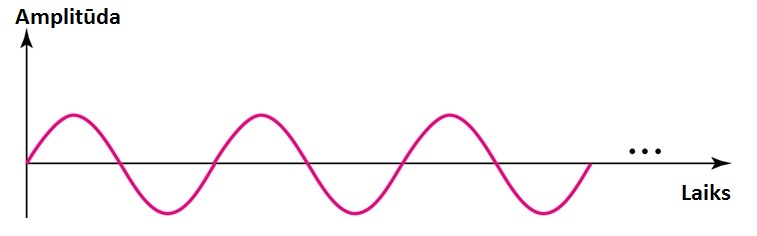
\includegraphics[width=0.70\textwidth]{sin} 
\caption{Sinusoīda \cite{properties}}  \label{sinusoida} 
\end{figure}

\subsection{Analoga signāla īpašības.}
\begin{itemize}
\item Periods ir laiks, kas nepieciešams, lai signāls veiktu  vienu svārstību ciklu no pozitīvām vērtībām uz negatīvām un atkal uz pozitīvām, līdz atkal sāks atkārtoties. Periods tiek mērīts sekundēs \cite{http://ecomputernotes.com/computernetworkingnotes/communication-networks/analog-signal} un to aprēķina izmantojot vienādojumu 
\begin{equation}
T = \frac{1}{f},
\end{equation}
kur 

$f$ - frekvence,

$T$ - periods.

\item Ar frekvenci saprot, cik  reizes vienā sekundē skaņas signāls no pozitīvām pāriet uz negatīvām un atkal uz pozitīvām vērtībām. Frekvenci mēra kā svārstību skaitu vienā sekundē jeb hercos (Hz) \cite{frequency}. Frekvence tiek aprēķināta pēc vienādojuma
\begin{equation}
f = \frac{1}{T},
\end{equation}
kur 

$T$ - periods,

$f$ - frekvence.

Vai arī pēc vienādojuma 
\begin{equation}
f= \frac{c}{\lambda},
\end{equation}
kur 

$f$ - frekvence,

$c$ - viļņa ātrums,

$\lambda$ ir viļņa garums \cite{http://www.sengpielaudio.com/calculator-period.htm}. 

Attēlā \ref{period} var novērot to, kā izmainās sinusoīdas periods atkarībā no frekvences.

\begin{figure}[H] \centering
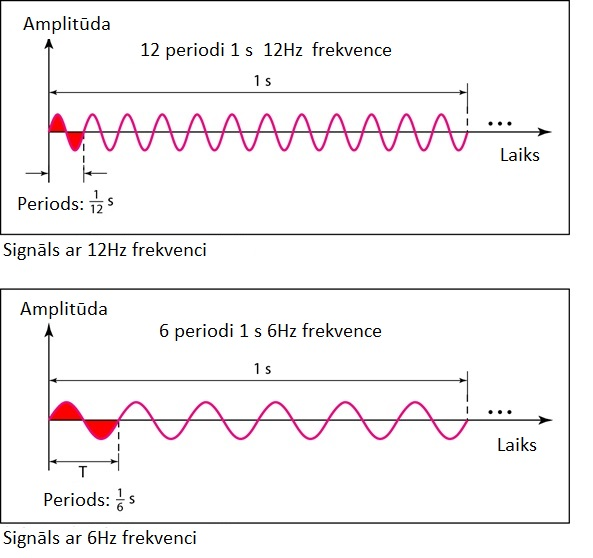
\includegraphics[width=0.65\textwidth]{frequency} 
\caption{Sinusoīda ar 12 Hz frekvenču (augšā), sinusoīda ar 6 Hz frekvenci (apakšā) \cite{properties}}  \label{period} 
\end{figure}

\item No amplitūdas ir atkarīgs skaņas signāla skaļums. Kad amplitūda ir lielāka, tad arī skaņas signāls ir skaļāks, bet kad amplitūda ir maza, signāls ir klusāks \cite{http://acad.carleton.edu/courses/musc108-00-f14/pages/01/01SixBasicPropertiesofSound.html}. Amplitūda ir maksimālā vai minimālā signāla vērtība līdz laika (x) asij. Amplitūda tiek mērīta decibelos (dB) \cite{http://computerrelatedinfo.blogspot.com/2012/12/what-is-analog-signal-its-properties.html}. Kā amplitūda ietekmē sinusoīdu var aplūkot attlēā \ref{amplitude}

\begin{figure}[H] \centering
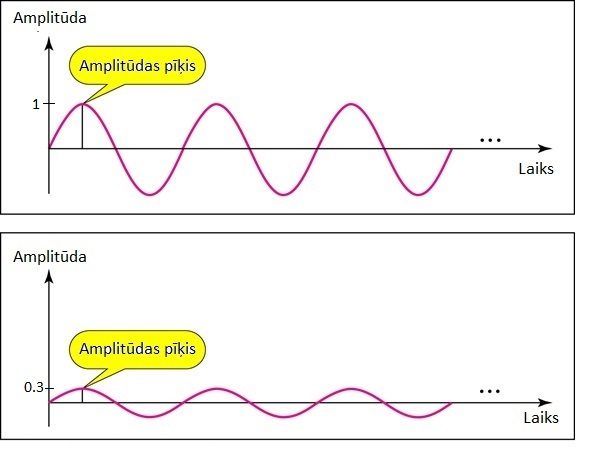
\includegraphics[width=0.65\textwidth]{amplitud} 
\caption{Sinusoīdas ar dažādām amplitūdām \cite{properties}}  \label{amplitude} 
\end{figure}

\item Tad vēl ir jāņem vērā arī fāze, kas raksturo signāla novirzi laika periodā 0, kas nosaka pirmā perioda stāvokli. Fāze tiek mērīta grādos vai radiānos \cite{http://ecomputernotes.com/computernetworkingnotes/communication-networks/analog-signal}. Attēlā \ref{phase} var novērot to, kā mainās sinusoīda laika periodā 0 atkarībā no fāzes novirzes. 

\begin{figure}[h] \centering
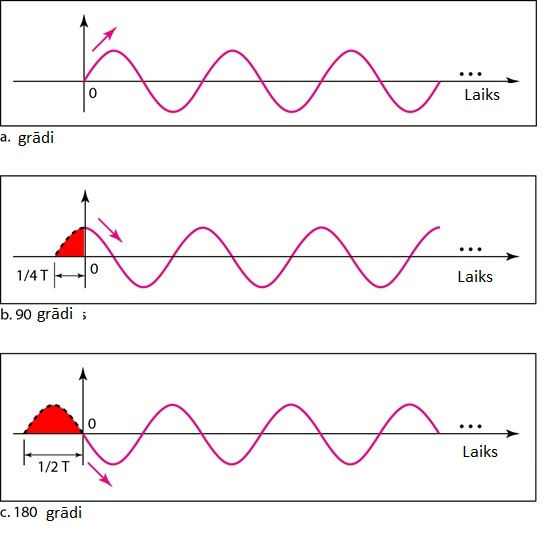
\includegraphics[width=0.65\textwidth]{phase} 
\caption{Sinusoīdas ar dažādām fāzēm \cite{properties}}  \label{phase} 
\end{figure}
\end{itemize}

\subsection{Diskrēts signāls}
\sloppy

Visi signāli, kas eksistē dabā ir analogi signāli, kā, piemēram, cilvēka runa, elektriskais signāls u.c. \cite{nature}, taču, lai varētu signālus reģistrēt un saglabāt datorā, nepieciešams skaņas signālus konvertēt uz digitāliem signāliem. Digitāliem signāliem ir daudz dažādu priekšrocību, kas saistās gan ar signālapstrādi, gan atmiņu, drošību u.tml. Vairāk par digitālā signāla priekšrocībām var uzzināt avotā \cite{adv}.  

Diskrēts signāls atšķirībā no analoga signāla satur noteiktu skaitu vērtību \cite{DiscreteSignal}. Izmantojot diskrētu signālu iespējams veikt dažādas operācijas, kā, piemēram, filtrēšanu bet jārēķinās ar to, ka ir iespējami datu zudumi un signāls var zaudēt savas rakstura iezīmes, ja tiek izvēlēti nepareizi parametri \cite{AnalogandDigitalSignal}.

\begin{itemize}

\item To cik daudz vērtības tiek ņemtas, lai rekonstruētu analogo signālu nosaka izgūšanas frekvence \cite{AnalogandDigitalSignal}. Ar izgūšanas frekvenci saprot to cik daudz vērtības tiek ņemtas no analogā signāla sekundē, lai to varētu pārveidot diskrētā signālā. Izgūšanas frekvence tiek mērīts hercos (Hz) \cite{http://www.digitizationguidelines.gov/term.php?term=samplingrateaudio}.

\item Pēc cik ilga laika tiek ņemts nākošais signāla intervāls nosaka izgūšanas periods. Izgūšanas periods ir laika intervāls start vienu vērtību un nākošo vērtību. Izgūšanas periodu nosaka pēc vienādojuma
\begin{equation}
Ts= \frac{1}{fs},
\end{equation}
kur 

$fs$ ir izgūšanas frekvence, 

$Ts$ ir izgūšanas periods. 

Izgūšanas periods tiek mērīts milisekundēs (ms) \cite{Sampling} . 

\end{itemize}

Attēlā \ref{sampling} var novērot to, ka palielinoties izgūšanas frekvencei samazinās izgūšanas periods un diskrētais signāls precīzāk reprezentē analogo signālu. Ir jābūt uzmanīgam cik lielu izvēlas izgūšanas frekvenci, jo kā var novērot attēlā \ref{sampling}  pēdējā grafikā, veidojas signāla kropļojums un signāls ir pilnībā izmanīts, kas notiek, kad ir izvēlēta pārāk maza izgūšanas frekvence un šo procesu var detalizētāk apskatīt avotā \cite{dtw52}.  
\FloatBarrier

\section{Izgūšanas (sampling) teorija}

Nyquist izgūšanas teorēma nosaka to cik lielai ir jābūt minimālajai izgūšanas frekvencei, lai izvairītos no signāla kropļojumiem. Teorēma nosaka, ka izgūšanas frekvencei ir jābūt vismaz divreiz lielākam par augstāko frekvenci signālā. To raksturo nevienādība 
\begin{equation}
f_s\geq  2f_c,
\end{equation}
kur 

$f_s$ ir izgūšanas frekvence,

$f_c$ ir augstākā frekvence signālā.

Ja izgūšanas frekvence ir lielāka, tad pietiek datu, lai rekonstruētu un netiktu izkropļots signāls, bet ja izgūšanas frekvence ir mazāka par esošo nevienādību tad, tiek ne tikai kropļoti un zaudēti signāla dati, bet arī pieļauj iespējamību, ka šos neprecīzos datus tālāk, kāds var izmantot un pat nenojaust to, kāds bija orģinālais signāls \cite{http://redwood.berkeley.edu/bruno/npb261/aliasing.pdf}. Attēlā \ref{sampling} pēdējā grafikā var novērot to, kā atšķiras orģinālais signāls no rekonstruētā signāla, kad ir izvēlēta pārāk maza izgūšanas frekvence. 

\begin{figure}[H] \centering
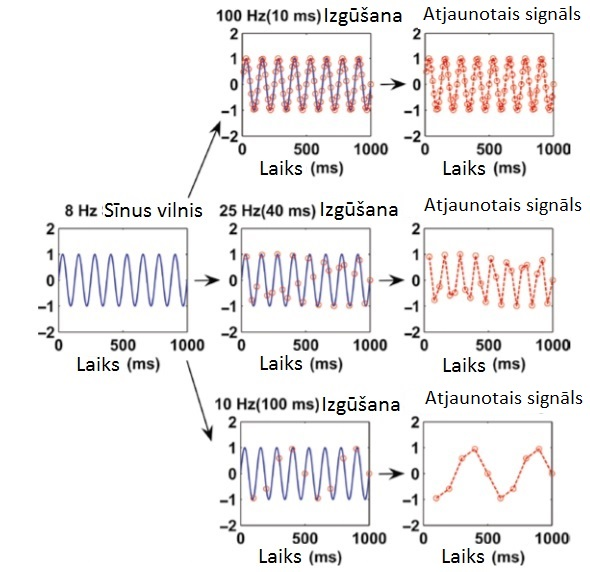
\includegraphics[width=0.80\textwidth]{sample} 
\caption{Analoga signāla transformācija diskrētā signālā izmantojot dažādas izgūšanas frekvences \cite{AnalogandDigitalSignal}}  \label{sampling} 
\end{figure}

\FloatBarrier
\section{Signāla reprezentācija laika telpā}
Var apskatīt doto skaņas signālu divās telpās - laika un frekvenču telpā. Abas telpas ir attēlotas attēlā \ref{domains}. 

\begin{figure}[H] \centering
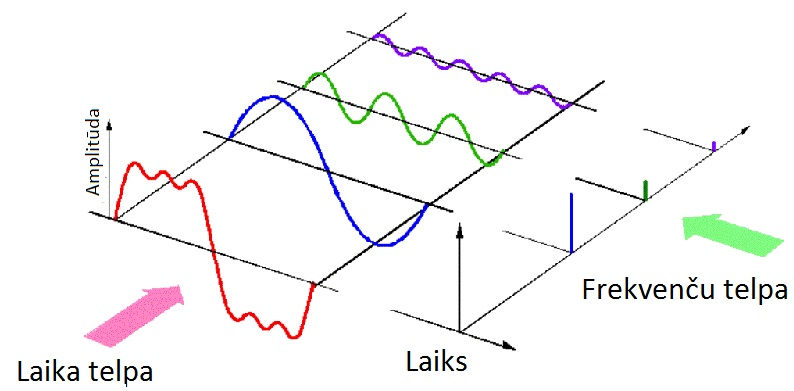
\includegraphics[width=0.60\textwidth]{up-sampling-fig3-lg} 
\caption{Sinusoīdas frekvenču un laika telpā \cite{domains}}  \label{domains} 
\end{figure}

\subsection{Laika telpa}

Laika telpā apskata signālu, kā laika (x ass) un amplitūdas (y ass) izmaiņas konkrētā laika momentā. Laika telpā, kamēr ir tikai vienkārša sinusoīda attēlā \ref{two-sinusoids},  ir iespējams prognozēt un saprast, kas notiek ar skaņas signālu. Bet kad runa ir par daudz sarežģītākiem signāliem, kā piemēram attēlā \ref{two-sinusoids} pa kreisi attēlotais signāls no divu sinusoīdu summa, paliek grūtāk saprast, kas notiek ar signālu, tāpēc ir nepieciešams pāriet uz frekvenču telpu, lai labāk varētu pētīt un salīdzināt skaņas signālus \cite{http://www.erzetich-audio.com/knowledgebase-05-time-vs-frequency}. Lai to izdarītu ir nepieciešams izmantot Furjē transformāciju, kuru apskata tālāk. 
\begin{figure}[H] \centering
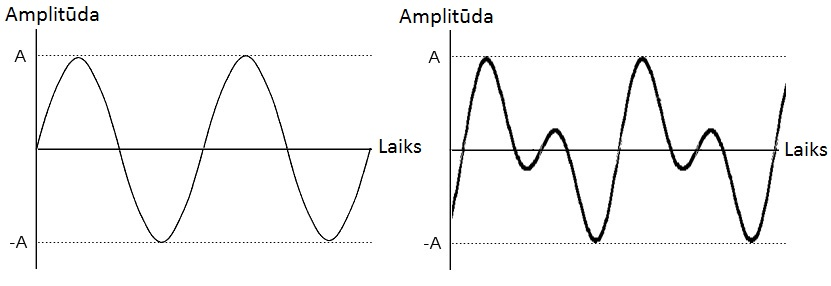
\includegraphics[width=0.65\textwidth]{soundsignals} 
\caption{Vienkārša sinusoīda (pa kreisi) un signāls no divu sinusoīdu summas (pa labi) \cite{http://www.erzetich-audio.com/knowledgebase-05-time-vs-frequency}}  \label{two-sinusoids} 
\end{figure}

\FloatBarrier
\subsection{Furjē teorēma} 

Franču matemātiķis un zinātnieks Jean-Baptiste Joseph Fourier ap 1800 gadu izveidoja teorēmu. Periodisku funkciju $f(x)$, kas ir nepārtraukta laikā, var izteikt kā daudzu sinusoīdu summu, kur katrai sinusoīdai ir sava specifiska amplitūda un fāzes koeficients (Furjē koeficients) \cite{Foure}. Kā veidojas sarežģīts signāls no sinusoīdu summas var aplūkot attēlā \ref{Fourier}. 
\begin{figure}[H] \centering
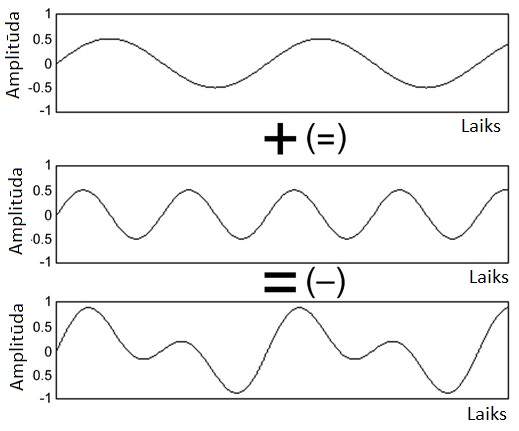
\includegraphics[width=0.50\textwidth]{sumofsines} 
\caption{Sarežģīta signāla izveide no divām sinusoīdām (no augšas uz apakšu) vai sadalīšana vienkāršās sinusoīdās (no apakšas uz augšu) \cite{Foure}}  \label{Fourier} 
\end{figure}

\FloatBarrier

\section{Signāla reprezentācija frekvenču telpā}

\subsection{Furjē transofrmācija}
Pielietojot Furjē transformāciju dekompozē sarežģītu skaņas signālu vienkāršās sinusoīdās, ko var apskatīt attēlā \ref{Fourier}, lai varētu skaņas signālu reprezentēt frekvenču telpā \cite{http://www.thefouriertransform.com/transform/fourier.php}. Matemātiski Furjē transformāciju, lai skaņas signālu attēlotu frekvenču telpā, raksturo ar vienādojumu:

\begin{equation}
F\{g(t)\}= G(f) = \int_{-\infty}^\infty g(t)e^{-2\pi ift} dt,
\end{equation}

kur 

g(t) - skaņas signāls laika momentā t,

f - frekvence,

t - laiks.

Zinot G(f), var pielietot inverso Furjē transformāciju, lai pārietu atpakaļ uz laika telpu \cite{http://www.thefouriertransform.com/transform/fourier.php}. 

\begin{equation}
F^{-1} \{G(f)\} = \int_{-\infty}^\infty G(f)e^{2\pi ift} df = g(t),
\end{equation}

kur 
G(f) - Sakņas signāls pie frekvences f

f - frekvence,

t - laiks.

Attēlā \ref{complex-signal} var apskatīt piemēru kā izskatās sarežģīts skaņas signāls laika un frekvenču telpā. 

Frekvenču telpa dod cita veida informāciju par skaņas signālu, kas sniedz ieskatu par to, kādas frekvenču komponentes ir pētāmajā signālā. Par frekvenču telpu tiks aprakstīts tālāk. 


\begin{figure}[H] \centering
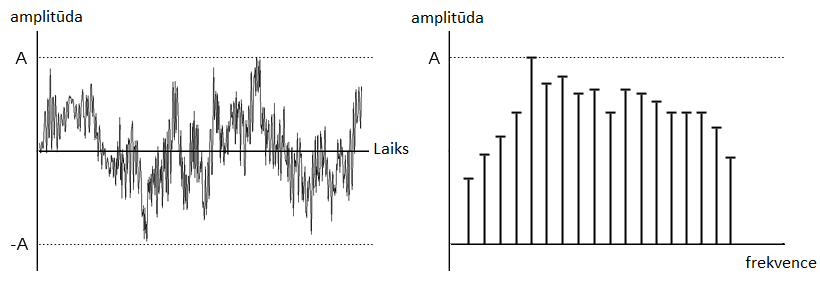
\includegraphics[width=0.70\textwidth]{act} 
\caption{Signāls laika telpā (pa kreisi) un frekvenču telpā (pa labi) \cite{http://www.erzetich-audio.com/knowledgebase-05-time-vs-frequency}}  \label{complex-signal} 
\end{figure}

\FloatBarrier
\subsection{Frekvenču telpa}


Atšķirībā no laika telpas, frekvenču telpā skaņas signāls tiek attēlots kā frekvences (x ass) un amplitūda (y ass) pie noteiktas frekvences. Attēlā \ref{time-frequency-signal} pirmajā grafikā var apskatīt skaņas signālu laika telpā, kas sastāv no divu sinusoīdu summas ar frekvencēm 4Hz un 12Hz un otrajā grafikā var redzēt šo pašu signālu tikai frekvenču telpā, kur atsevišķi tiek attēlotas abu sinusoīdu frekvences un amplitūdas \cite{http://www.theparticle.com/cs/bc/mcs/signalnotes.pdf}.

\begin{figure}[H] \centering
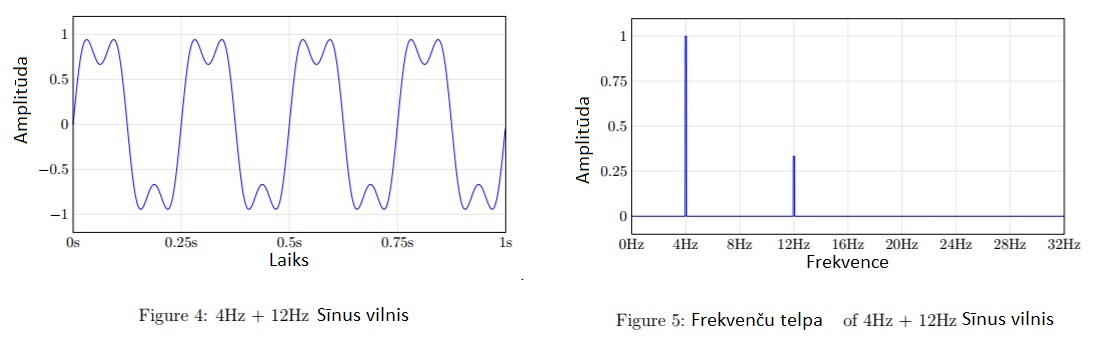
\includegraphics[width=0.90\textwidth]{timeAndFrequencyDomain} 
\caption{Signāls no divu sinusoīdu summas (pa kreisi) un sinusoīdas frekvenču telpā  \cite{http://www.theparticle.com/cs/bc/mcs/signalnotes.pdf}}  \label{time-frequency-signal} 
\end{figure}
  
\FloatBarrier
\section{Signāla reprezentācija laika/frekvenču telpā}
\subsection{Spektrogramma}


Spektrogramma ir veidota no secīgiem spektriem, apvienojot tos kopā laikā un saspiežot amplitūdas asi uz "kontūru kartē", kas uzzīmēta uz izlozētas
pelēkās skalas. 
Gala grafikā ir laiks, pa horizontālo asi, frekvenci gar
vertikālās ass, un signāla amplitūda jebkurā laika brīdī un frekvence tiek parādīta kā
pelēks līmenis. Tradicionāli, melns tiek izmantots, lai norādītu uz vislielākajām enerģijām, bet baltais tiek izmantots
lai attēlotu mazākās enerģijas.

Klusuma mirkļi un momenti, kad frekvenču enerģija ir maza, spektrogrammā tiek attēloti ar baltu krāsu. Tumšie laukumi attēlo enerģijas apgabalus, kurus 
izraisa balss saišu sašaurināšanās, harmonikas vai formantu vibrācijas skaņas signālā.  \cite{dtw21}

Spektrogrammu var aplūkot attēlā \ref{spectogram-gray}. Noteiktas frekvences tiek uzsvērtas un tās var redzēt kā horizontālas līnijas vai neregulārus svītrojumus. Šīs uzsvērtās frekvences sauc par formantām, par kurām tiks runāts tālāk \cite{Acoustic}.
Spektrogrammas izveides pamatā ir īsā laika Furjē transformācija \cite{dtw22}.

\begin{figure}[H] \centering
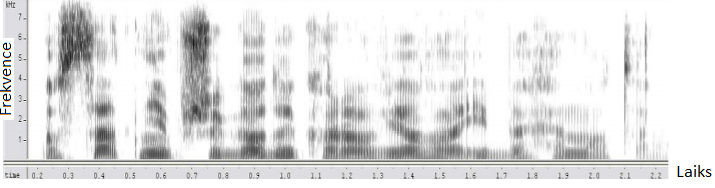
\includegraphics[width=0.90\textwidth]{spectogramm} 
\caption{ Spektrogramma \cite{Acoustic}}  \label{spectogram-gray} 
\end{figure}

Runas pētījumos tiek izmantotas divu veidu spektrogrammas:
\begin{itemize}

\item Spektrogramma, kas uzsver frekvenču
aspektus, izmantojot šauras analīzes filtrus \cite{dtw21}. Šaurjoslas spektrogrammas ir ērtas, lai izpētītu skaņas avota rakstura iezīmes. Tās parāda harmonikas, kas rodas no balss saišu vibrācijas.

\item Spektrogramma, kas uzsver īslaicīgus aspektus, izmantojot platas analīzes filtrus \cite{dtw21}. Platjoslas spektrogrammas ir ērtas, lai izpētītu vokālā trakta filtru īpašības. Tās izceļ vokālā trakta rezonanses (formants) \cite{dtw21}. 

\end{itemize}
Sieviešu balsīs ir vairāk frekvenču komponentes nekā vīriešu un parasti sievietes balsī dominē augstākās frekvences, bet vīrieši balsī dominē zemās frekvences \cite{FMVoice}. Tas ir attēlots spektrogrammās \ref{fm-m}, kur frekvenču intensitāte tiek attēlota uz vertikālās ass, bet laiks uz horizontālās ass.
No spektrogrammas datiem var veikt labu signāla analīzi, kur var noteikt skaņas signāla ilgumu, fonētiskās īpašības kā arī var identificēt dažādas skaņas, ņemot vērā formantas, vokālā trakta izmaiņām, kad pāriet no vienas skaņas uz otru, kā arī vokālā trakta pulsāciju \cite{http://www.cslu.ogi.edu/tutordemos/SpectrogramReading/spectrogram.html}.

\begin{figure}[H] \centering
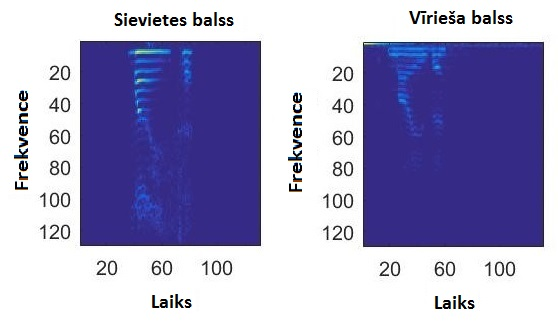
\includegraphics[width=1.00\textwidth]{spectr} 
\caption{Sievietes balss platjoslas spektrogramma (pa kreisi) un vīrieša balss platjoslas spektrogramma (pa labi) ierunājot vārdu "maize" 
\cite{matlab}} \label{fm-m} 
\end{figure}


\chapter{Skaņas signāla apstrāde}



\section{Digitālā laika deformācija}

Vienu vārdu ir iespējams izrunāt dažādi. Vārdi var atšķirties no tā, kas tos izrunā, kā tie tiek izrunāti – ātrāk, lēnāk, skaļāk, klusāk. Jāņem vērā arī tas, ka vārdi, burti, skaņas utt. tiek izrunātas dažādos laika momentos. Lai spētu salīdzināt cik lielā mērā viens skaņas signāls atšķiras no otra ir nepieciešams veikt digitālo laika deformāciju. 

Digitālā laika deformācija tiek izmantota automātiskās runas atpazīšanā, lai savstarpēji salīdzinātu divus laikā atšķirīgus skaņas signālus \cite{DynamicTimeWrapping}.
Tiek apskatīts digitālās laika deformācijas piemēru, kur ir divi diskrēti signālu vektori ar vērtībām $X: = \{p_1,p_2,…p_N\}$ un ar garumu N un $Y:= \{q_1,q_2,…q_M\}$ ar garumu M. Abu signālu vērtības tiek ņemtas ekvivalenti vienādos laika momentos, ko var apskatīt attēlā \ref{different-time-intervals}. 

\begin{figure}[H] \centering
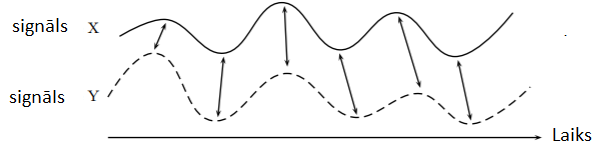
\includegraphics[width=0.70\textwidth]{dtw} 
\caption{Divu signālu novietojums laikā momentā. Signālu izlīdzinātie punkti tiek savienoti ar bultām \cite{DynamicTimeWrapping}}  \label{different-time-intervals} 
\end{figure}

Tālāk ir nepieciešams atrast kartografēšanas ceļu $\{(p_1,q_1),(p_2,q_2),...,(p_k,q_k)\}$ , tā lai distance kartografēšanas ceļā 

\begin{equation}
\sum\limits^k_{i=1} |X(p_i)−Y(q_i)|,
\end{equation}

kur 

$X(p_i)$ - X vektora attiecīgais elements,

$Y(q_i)$ - Y vektora attiecīgais elements,

k - kopējais elementu skaits,


 tiktu minimizēta. Kā izskatās kartografēšanas ceļš var redzēt attēlā \ref{cost-matrix}. 

\begin{figure}[H] \centering
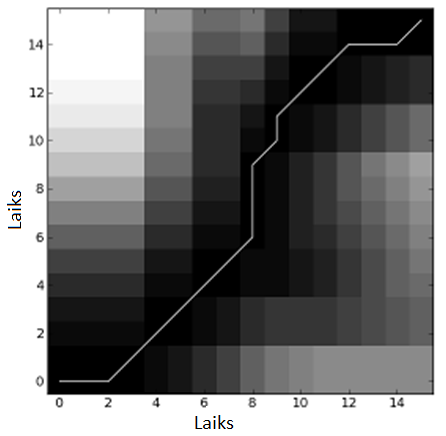
\includegraphics[width=0.50\textwidth]{pathdtw} 
\caption{Kļūdas matrica starp diviem signāliem \cite{dtw1}}  \label{cost-matrix} 
\end{figure}

Veidojot kartografēšanas ceļu nepieciešams ievērot divus nosacījumus.

\begin{itemize}

\item Nepieciešams uzstādīts sākuma nosacījums $(p_1,q_1)=(1,1)$ un beigu nosacījums $(p_k,q_k)=(m,n)$, lai ierobežotu kartografēšanas ceļa laukumu.
\item Tiek noteiks, katra mezgla (i,j) iespējamais kustības laukums uz citiem mezgliem (i−1,j), (i,j−1), (i−1,j−1). Šo nosacījumu var redzēt attēlā \ref{road}. Šīs ierobežojums garantē to, ka kartēšana ceļš monotoni nesamazinās tās pirmajos un otrajos argumentos. Turklāt jebkuram elementam X vektorā, vajadzētu spēt atrast vismaz vienu atbilstošu elementu Y vektorā, un otrādi.

\end{itemize} 

\begin{figure}[h] \centering
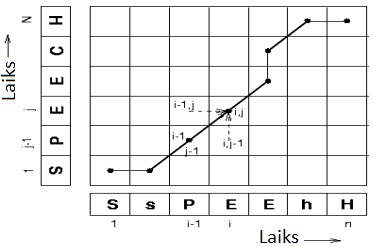
\includegraphics[width=0.90\textwidth]{rules} 
\caption{Deformācijas ceļš \cite{dtw2}}  \label{road} 
\end{figure}

Pēc tam nepieciešams pielietot uz priekšu veicamo laika deformāciju ievērojot šos soļus:
\begin{enumerate}

\item Vispirms nepieciešams inicializēt matricu D(n$\times$m) un pēc tam tā jāaizpilda ar sākuma vērtībām, nodefinējot D(i,j) kā distanci starp x(1:i) un y(1:j) un aizpildot ar vērtībām no kartografēšanas ceļa kas sākas no (1,1) līdz (i,j).
\item Tad jāpielieto rekursijas formula (1), lai varētu aizpildīt visu matricu D ar jaunām vērtībām ievērojot sākuma nosacījumu (1):
\item Un tad iegūst matricu D(m,n) ar vērtībām, kas raksturo signālu, kurš ir ticis deformēts laikā. To var apskatīt attēlā \ref{dynamic-time}, kur ar sarkano līniju atspoguļo signālu, kas tiek deformēts laikā, lai sakristu ar signālu ,kas apzīmēts ar zilo līniju. 

\end{enumerate}

\begin{figure}[H] \centering
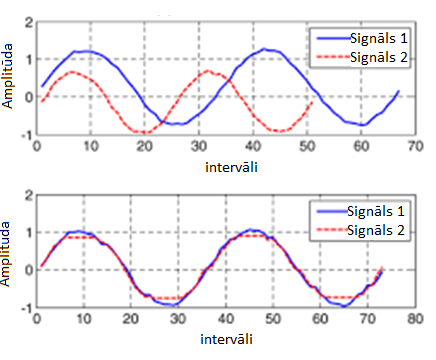
\includegraphics[width=0.70\textwidth]{asdd} 
\caption{Divi signāli (augšā) un šie signāli pēc digitālā laika deformācijas pielietošanas (apakšā) \cite{dtw3}}  \label{dynamic-time}
\end{figure}

Kad esam veikuši DTW \cite{DTWalgoritm}, pirms salīdzināt cik lielā mērā signāli ir līdzīgie viens otram, nepieciešams izgūt abu signālu raksturojošās īpašības. Metodes, kā veikt šo īpašību izgūšanu tiks aprakstīts tālāk. 
\FloatBarrier

\section{Trokšņi}
Troksnis ir nevēlama parādība skaņas signālā, kas veic skaņas signāla degradāciju. Tomēr nelieli trokšņi signālā ir pieņemami un pat vēlami, kā piemēram, baltie trokšņi, kas tiks aprakstīti tālāk \cite{Noises}.
Bet ja troksnis ir pārāk liels, tad pastāv iespējamība, ka signāls tiek bojāts tik ļoti, ka dati vairs nav izmantojami \cite{Pacienta-runas-kvalitātes-noteikšanas-automatizētas-sistēmas-izstrāde}.
Ierunājot skaņas signālu fona trokšņi var rasties dažādu iemeslu dēļ, piemēram, runātāja mikrofons var radīt traucējumus, elektroniskus trokšņus vai arī kamēr tiek ierunāts skaņas signāls paralēli notiek citas darbības, kas var radīt fona skaņas u.c. \cite{noi1}. 

Lai samazinātu trokšņus skaņas signālā, ir nepieciešams veikt trokšņu filtrāciju, kas minimizētu radītos trokšņus, atstājot tikai nepieciešamos runātāja datus. Kā izskatās signāls ar troksni un pēc trokšņa filtrācijas var apskatīt attēlā \ref{nois}. Tomēr ar filtrāciju ir jābūt uzmanīgiem, jo filtru pielietošana var būtiski uzlabot skaņas signālu, vai arī tieši pretēji, izmantojot nepiemērotus parametrus var zaudēt signālā esošo un derīgo informāciju to kropļojot \cite{https://www.nde-ed.org/EducationResources/CommunityCollege/EddyCurrents/Procedures/SignalFiltering.htm}.

Ir jāapskata arī tāds termins kā signāla-trokšņa attiecība. SNR salīdzina skaņas signāla enerģijas līmeni ar trokšņa enerģiju. Un tas tiek visbiežāk izteikts decibelos (dB). Jo lielāka vertība ir SNR, jo vairāk signāls satur noderīgu informāciju, nekā nevēlamus datus jeb troksni \cite{https://www.lifewire.com/signal-to-noise-ratio-3134701}.


\begin{figure}[H] \centering
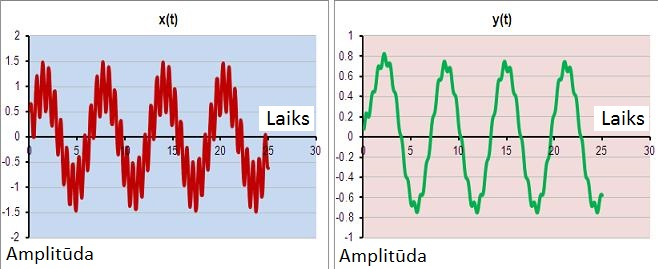
\includegraphics[width=0.80\textwidth]{LowPass} 
\caption{Signāls ar trokšņiem (pa kreisi) un signāls, kam veikta trokšņu filtrācija (pa labi) \cite{dtw4}}  \label{nois} 
\end{figure}

\FloatBarrier

\subsection{Skaņas signāla enerģija}
Enerģiju signālā aprēķina ar vienādojumu \cite{energy}:
\begin{equation}
E = \int^\infty_{- \infty}|x(t)|^2dt,
\end{equation}

kur

$E$ - signāla enerģija,

$t$ - laiks,

$x$ - skaņas signāls,

$x(t)$ - skaņas signāls laika momentā t.

Diskrētam skaņas signālam aprēķina enerģiju ar vienādojumu :
\begin{equation}
E = \sum^\infty_{n =- \infty}|x(t)|^2dt,
\end{equation}

kur

$E$ - signāla enerģija,

$t$ - laiks,

$x$ - skaņas signāls,

$x(t)$ - skaņas signāls laika momentā t.


\subsection{Baltie trokšņi}
Baltais troksnis ir nejaušs signāls, kas satur dažādas frekvences ar vienādu intensitāti piešķirot signālam nemainīgu spektrālo blīvumu \cite{wiki}. 
Baltā trokšņa grafisko attēlojumu var redzēt attēlā \ref{white-noise} Un baltā trokšņa process ${W(t)}$ tiek aprakstīts ar vienādojumu

\begin{equation}
S_W(\omega)=\frac{N_0}{2}, kur
 -\infty < \omega < \infty ,
\end{equation}

kur 

$N_0$ ir konstante un to sauca par baltā trokšņa intensitāti,

$S_W(\omega)$ - enerģijas spektrālais blīvums \cite{dtw46}. 
%(http://www.ece.tufts.edu/~maivu/ES150/8-lti_psd.pdf)
%(http://www.ece.iit.edu/~biitcomm/research/references/Other/Tutorials%20in%20Communications%20Engineering/TUTORIAL%201%20-%20Basic%20concepts%20in%20signal%20processing.pdf)



Vidējo baltā trokšņa spēku aprēķina izmantojot formulu 
%(http://www.ece.uah.edu/courses/ee385/500ch8.pdf)
\begin{equation}
P_{avg} =\frac{1}{2 \pi } \int^{\infty}_{ -\infty } S_W(\omega) d \omega \rightarrow \infty ,
\end{equation}

kur 

$P_{avg}$ - Vidējais baltā trokšņa spēks,

$S_W(\omega)$ ir enerģijas spektrālais blīvums.



Var teikt, ka baltie trokšņi ir matemātiska abstrakcija un balto trokšņu procesu nevar paredzēt, tāpēc, ka trokšņu paraugi dažādos laika momentos ir nekorelēti, lai arī cik tuvu paraugi neatrastos viens otram \cite{WhiteNoise}. 

Var izmantot baltos trokšņus sintētisko skaņas signālu izveidē, lai iegūtie paraugi vairāk atšķirtos viens no otra. Gausa baltais troksnis ir pamata trokšņu modelis, kuru izmanto, lai imitētu dažādu procesu efektu, kas notiek dabā.
\begin{itemize}

\item Gausa balto troksni var pievienot jebkuram troksnim, kas var būt raksturīgs attiecīgai informācijas sistēmai. 
\item Baltais apzīmē to, ka tam piemīt vienāda enerģija pie visām frekvencēm spektrā. 
\item Gausa apzīmē to, ka tam ir normāls sadalījums laika telpā ar nulles vidējā laika telpas vērtību \cite{wiki}
\cite{http://www.nosleeplessnights.com/what-is-white-noise-whats-all-the-fuss-about/}. 
\end{itemize} 

\begin{figure}[H] \centering
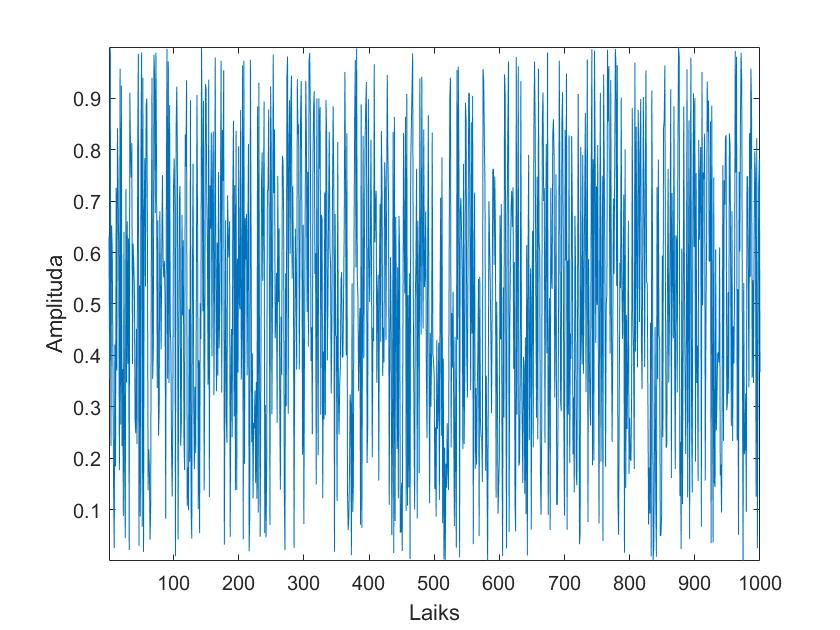
\includegraphics[width=0.65\textwidth]{white} 
\caption{Ģenerēts Gausa baltais troksnis izmantojot MATLAB \cite{Noises}}  \label{white-noise} 
\end{figure}

\section{Filtrēšana}
Filtrēšanu pielieto, kad nepieciešams atbrīvoties no nevēlamas informācijas signālā. Filtrēšanā izņem dažas frekvences, bet citas atkal atstāj, lai samazinātu fona trokšņus, vai citus nevēlamus signālus. Ideālajā gadījumā filtram nevajadzētu pievienot jaunas frekvences vai mainīt frekvenču komponentes signālā, bet filtrs mainīs dažādu frekvenču komponenšu relatīvās amplitūdas un iespējams mainīs signālu fāžu attiecības \cite{http://www.ti.com/lit/an/snoa224a/snoa224a.pdf}. 
Piemēram ir dots signāls ar frekvenci $f_1$ un tad ir vēl signāls ar frekvenci $f_2$, kas rada nevēlamas skaņas, nepieciešams izfiltrēt nevēlamo signālu. 
Filtrs var tikt parādīts kā koeficientu reizinājums ar konkrētām frekvencēm. Pareizinot ar 1, nemainās, taču ar 0.1 tiek samazināta šīs frekvences nozīme signālā, līdz ar to attiecīgā frekvence tiek zaudēta (nofiltrēta).
 Šo procesu var apskatīt attēlā \ref{filtering}, kur novērojams ka tiek samazināts signāls ar frekvenci $f_2$, kas ir nevēlams signāls, kamēr patur nemainīgu signālu ar frekvenci $f_1$, kas nepieciešams tālākai analīzei un apstrādei. 

\begin{figure}[H] \centering
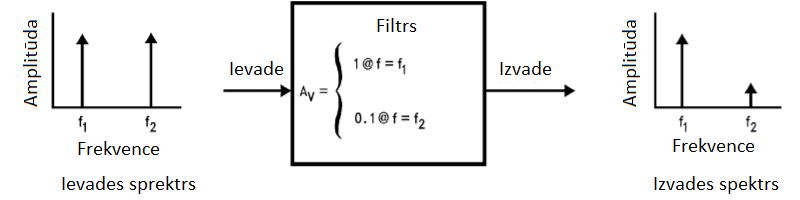
\includegraphics[width=1.00\textwidth]{filtering} 
\caption{Nevēlamā signāla ar frekvenci $f_2$ un nepieciešamā signāla ar frekvenci $f_1$ filtrācija \cite{http://www.swarthmore.edu/NatSci/echeeve1/Ref/DataSheet/IntroToFilters.pdf}}  \label{filtering} 
\end{figure}

Pastāv dažāda veida filtri.
\begin{itemize}

\item Zemfrekvenču filtrs attēlā \ref{filtr}, kuru pielieto, lai tiktu atstātas zemās frekvences un izfiltrētas augstās frekvences. Šis filtrs atmet visas frekvences, kas ir augstākas par atmešanas sliekšņa frekvenci \ref{filtr}.  

\item Augstfrekvenču filtrs attēlā \ref{filtr}, kuru pielieto, lai veiktu zemo frekvenču filtrāciju. Šis filtrs atmet visas frekvences, kas ir zemākas par nogriešanas frekvenci \ref{filtr}. 

\item Joslu caurlaides filtrs attēlā \ref{filtr}, kas izfiltrē noteiktas augstās un zemās frekvences atstājot noteiktu frekvenču intervālu u.c. filtri \cite{http://www.swarthmore.edu/NatSci/echeeve1/Ref/DataSheet/IntroToFilters.pdf}. 

\end{itemize}
\begin{figure}[H] \centering
\includegraphics[width=1.02\textwidth]{bandPassFilter} 
\caption{ Joslu caurlaides filtrs (pa kreisi), Augstfrekvenču filtrs (pa vidu), Zemfrekvenču filtrs (pa labi) \cite{dtw6}}  \label{filtr} 
\end{figure}


\subsection{Vīnera Filtrs} 
Vīnera filts ir lineāri laikā nemainīgs (no angļu val. linear time invariant jeb LTI), kas paredzēts nejaušiem, stacionāriem procesiem, kurus degradējis troksnis ar zināmiem vai noteiktiem trokšņā parametriem. Vīnera filtru pielieto frekvenču domēnā. 

Kā piemēru apskatīsim šī filtra pielietojumu attēlu apstrādē.
Ja ir dots degredēts attēls $x(n,m)$, tiek pielietota 
DFT un iegūts $X(u,v)$. Orģinālās bildes spektrs tiek aprēķināts
izmantojot $X(u,v)$, kam pievienots Vīnera filtrs \cite{dtw45}:

\begin{equation}
\hat{S}(u,v) = G(u,v)X(u,v),
\end{equation}

kur 

$\hat{S}(u,v)$ - Orģinālās bildes spektrs,

$G(u,v)$ - Vīnera filtrs,

$X(u,v)$ - Bilde pēc DFT pielietošanas.

Inversā DFT tiek pielietota, lai iegūtu paredzēto bildi no tās spektra. Vīnera filtru raksturo šāds vienādojums:

\begin{equation}
G(u,v) = \frac{H\times(u,v)P_s(u,v)}{|H(u,v)|^2P_s(u,v)+P_n(u,v)},
\end{equation}

kur

$H(u,v)$ - Punktu izplatījuma funkcijas Furjē transformācija \cite{pftdft}. Punkta izplatījuma funkcija ir veids kā aprakstīt kā punkts izplata savu enerģiju sev apkārt divdimensionālā telpā. Par punktu izplatījuma funkciju detalizētāk var uzzināt avotā \cite{points},

$P_s(u,v)$ - Signāla enerģijas spektrs, kas tiek iegūts aprēķinot signāla auto korelācijas Furjē transformāciju, 

$P_n(u,v)$ - Trokšņu procesa enerģijas spektrs, kas tiek iegūts ņemot trokšņa auto korelācijas Furjē transformāciju.




\section{Klusumu intervālu izņemšana}
Signāla intervālu, kas nesatur runātāja balss informāciju, raksturo neperiodiska un trokšņa veida daba, kā arī relatīvi zema enerģija salīdzinājumā ar intervālu, kur ir runa. Šajā signālā intervālā ir vairāk nulles līmeņa šķērsošanas jeb momenti, kad signāls mainās no pozitīvām uz negatīvām vai no negatīvām atbakaļ uz pozitīvām vērtībām, kā arī relatīvi maza korelācija starp secīgiem signāla intervāliem. Signāla intervāls, kur nav runa tiek identificēts laika telpā savu īpašību dēļ. Bet frekvenču telpā, ja nav harmoniskas struktūras noteiktam segmentam, tad var secināt, ka tur nav runas informācijas \cite{http://iitg.vlab.co.in/?sub=59&brch=164&sim=613&cnt=2}.

Klusuma izņemšanu var apskatīt attēlā \ref{silence}, kur izņem ārā tās signāla daļas, kur ir klusuma brīži ar nenozīmīgiem fona trokšņiem, lai atstātu tikai datus, kas satur runātāja balsi, jo nav īpaši nekādas jēgas no skaņas  fragmentiem, kas nesatur nekādu informāciju par runātāja balsi. Tas tikai palēnina skaņas signālu salīdzināšanu, jo salīdzināšanas procesā tiek apstrādāti un salīdzināti arī fragmenti, kas sevī ietver tikai nelielus fona trokšņus \cite{http://www.asha.org/policy/GL1988-00008.htm}.

Lai izņemtu klusumus un saglabātu runātāja balsi, pielieto dažādus algoritmus. Vispopulārākās ir īsa laika enerģija un nulles līmeņa šķērsošanas biežums(no angļ. val. zero crossing rate) jeb cik reizes signāls mainās no pozitīvām uz negatīvām vai no negatīvām atbakaļ uz pozitīvām vērtībām \cite{zerocross}. Tiek pieņemts, ka fona trokšņiem, kas ir signālā piemīt Gausa trokšņu raksturs. Galvenais ir jānosaka slieksnis starp runātāja balsi un troksni, lai varētu izņemt tos intervālus, kur nav runātāja balss informācija.
Parasti pirmās 200 milisekundes vai vairāk signālā tiek ierakstīts fona trokšņus vai klusumu, jo runātājam nepieciešams neliels laika brīdis pirms viņš ierunā attiecīgo skaņu, vārdu vai frāzi \cite{noise1}.
Ņemot vērā šo pieņēmumu var veikt attiecīgās darbības, lai izņemtu klusumus un fona trokšņus: 
\begin{enumerate}

\item Aprēķināt vidējo $\mu$ un standarta novirzi $\sigma$ pirmajām 200ms no attiecīgā skaņas signāla.

\item Nepieciešams apskatīt no pirmā līdz pēdējam signāla intervālam skaņas signālā un pārbaudīt katram signāla intervālam, vai Mahanalobis distance ir lielāka par 3 jeb: 

\begin{equation}
\frac{|x-\mu|}{\sigma}>3,
\end{equation}

kur

$\mu$ - vidējā novirze,

$\sigma$ - standarta novirzi,

$x$ - attiecīgā signāla intervāls,

$3$ - slieksnis, kas reprezentē standarta noviržu skaitu, kuru iegūst balstoties uz Gausa sadalijuma vienādojuma \ref{eq: gaus}.

Ja izpildās nevienādība tad signāla intervāls satur runātāja balsi bet ja nē tad šis signāla intervāls ir fona troksnis vai klusums. Slieksnis noraida paraugus līdz 99,7\% balstoties pēc Gausa sadalījuma vienādojuma

\begin{equation}\label{eq: gaus}
P[|x−\mu|\leq3\sigma];0.997,
\end{equation}
kur 

$P$ - varbūtība,

$\mu$ - vidējā novirze,

$\sigma$ - standarta novirzi,

$x$ - attiecīgā signāla intervāls,


tādējādi pieņemot tikai signāla intervālus, kas satur runātājā balsi.
\item Atzīmē intervālus, kas satur runātāja balsi kā 1, bet ,kas nesatur runātāja balsi, kā 0. Sadala visu skaņas signālu 10 ms nepārklātos logos. Skaņas signāls tādējādi tiek reprezentēts kā nulles un vieninieki.
\item Pieņem, ka ir M nulles un N vieninieki logā. Ja $M \geq N$ tad vieniniekus konvertē uz 0 un otrādi. Šī nevienādība tiek pielietota, paturot prātā, ka runa, kas veidojas no balss saitēm, mēles, vokālā trakta utt., nevar pēkšņi nelielā laika brīdī izmainīties, ņemot ka tās ir 10 ms.
\item Ņem tikai daļas no loga masīva, kas sastāv no runātāja balss un ievieto jaunā masīvā. Un tad iegūst tikai runātāja balsi bez citas liekas informācijas \cite{noise1}. 

\end{enumerate}

\begin{figure}[H] \centering
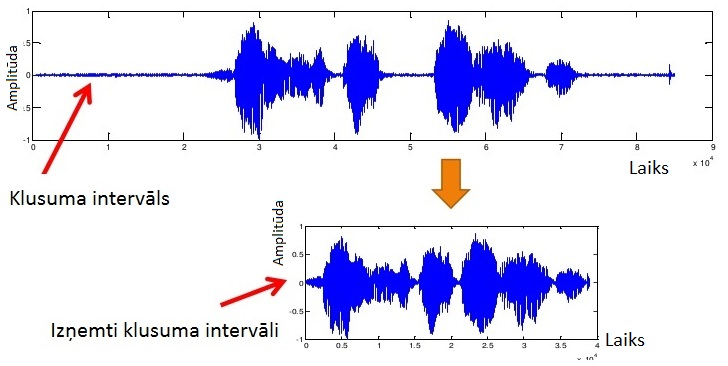
\includegraphics[width=1.00\textwidth]{silent} 
\caption{Orģinālais signāls (augšā) un signāls, kam veikta klusumu izņemšana (apakšā) \cite{dtw8}}  \label{silence} 
\end{figure}

Detalizēti iepazīties ar algoritmu iespējams avotā \cite{dtw24}.

\chapter{Skaņas signāla modelēšana}

\subsubsection{Harmonikas}
Lai saprastu, kas ir harmonikas jāsāk ar fundamentālo frekvenci.

Par fundamentālo frekvenci sauc zemāko rezonanses frekvenci un apzīmē kā $F_0$. Pieaugušam cilvēkam $F_0$ variē no 100 – 300 Hz.  
Zinot $F_0$, ir iespējams atrast harmonikas pēc formulas 
\begin{equation}
H(k)=k \times F_0,
\end{equation}
kur 

$k$ ir harmonika, kuru vēlamies atrast,

$F_0$ ir fundamentālā frekvence,

$H(k)$ ir harmonika.

Harmonikas, nevar sadzirdēt kā atsevišķus toņus, jo harmonikām ir daudz zemākas amplitūdas nekā fundamentālām frekvencēm, ko var apskatīt attēlā \ref{harmonic}  \cite{https://underlingsosu.wordpress.com/2013/03/08/phonetics-phriday-fundamental-frequency-harmonics-and-formant-frequencies/}. Toties tās piešķir balsij īpatnējās rakstura iezīmes \cite{http://person2.sol.lu.se/SidneyWood/praate/whatform.html}. 

\begin{figure}[H] \centering
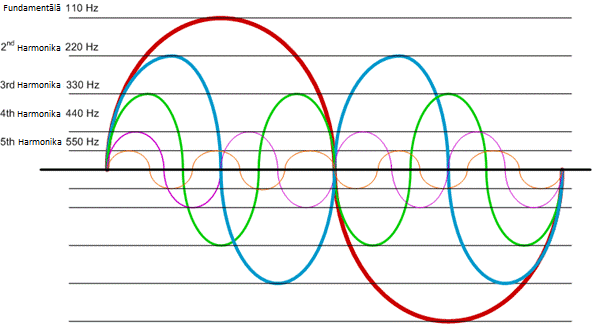
\includegraphics[width=0.90\textwidth]{Harmonic} 
\caption{Ar sarkano līniju attēlo fundamentālo frekvenci, bet ar parējām attēlo harmonikas \cite{dtw10}}  \label{harmonic} 
\end{figure}

Harmonikas, kuru frekvences ir tuvu vokālā trakta rezonanses frekvencei, brīvi iziet cauri vokālajam traktam radot formantu. Bet citas harmonikas neiziet cauri vokālajam traktam un šis harmonikas tiek novājinātas \cite{http://person2.sol.lu.se/SidneyWood/praate/whatform.html}.  

\section{Formantas}

Formantas pēc savas būtības ir akustiskas rezonanses cilvēka vokālajā traktā. Tās ir fiziskas īpašības, kas tiek sasaistītas ar katru patskani. Mēlei mainot savu pozīciju, tiek mainīta vokālā trakta forma un tādēļ arī mainās formantas. Tā kā mēle var kustēties nepārtraukti mainot savu pozīciju, arī formantu frekvences mainās nepārtraukti, katra savā individuālajā intervālā. Katrai valodai specifiski mainās mēles pozīcija izrunājot skaņas un tāpēc arī katrai valodai ir specifiskas formantu frekvences \cite{voice}.

Pastāv vairākas formants, kas veidojas katra pie noteiktām frekvencēm. Formanta veidojas aptuveni ik pēc 1000Hz intervāla. Formantas numurē secīgi, sākot ar zemāko rezonanses frekvenci  \cite{http://person2.sol.lu.se/SidneyWood/praate/whatform.html}. Attēlā \ref{formantas2} var apskatīt formantu secīgu numerāciju.


Pirmajai formantai ir 300-1200Hz plašs frekvenču diapazons. Otrajai formantai ir 800-3000Hz liels diapazons. Pārējām formantām ir salīdzinoši daudz mazāks diapazons. Formantas nevar mainīties individuāli, bet noteiktās kombinācijās \cite{voice}. 

Izmantojot tikai formantas var klasificēt visus patskaņus, ko cilvēka var izrunāt. Tas arī dod iespēju izmantojot formantas radīt sintētiskus skaņas signālus. Lielākoties izmanto tikai formantas $F_1$ un $F_2$, lai radītu patskaņus. Angļu valodas patskaņu formantu $F_1$ un $F_2$ vērtības var apskatīt attēlā \ref{formantas3}. Bet kopumā ir 4 formantas, kas veido katru patskani \cite{https://makarandtapaswi.wordpress.com/2009/08/30/time-and-frequency-formants-and-harmonics/}.
 
Spektrogrammā \ref{formantas1} var apskatīt formantas, kas iezīmētas ar sarkanu krāsu.

\begin{figure}[H] \centering
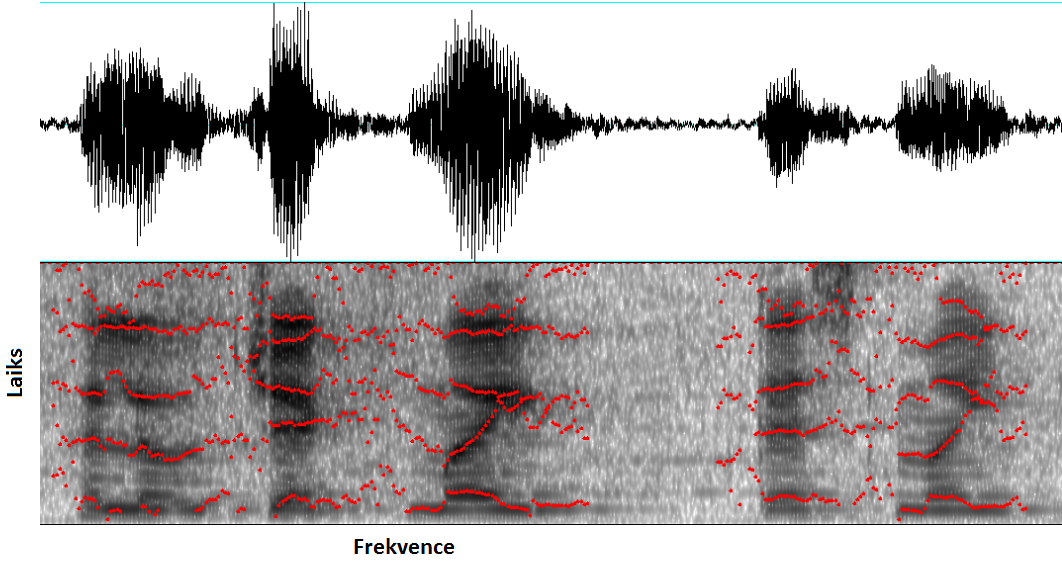
\includegraphics[width=0.70\textwidth]{formants} 
\caption{Skaņas signāls (augšā) un signāla spektrogramma, kur attēlotas formantas ar sarkano līniju(apakšā) \cite{https://makarandtapaswi.wordpress.com/2009/08/30/time-and-frequency-formants-and-harmonics/}}  \label{formantas1} 
\end{figure}

Protams ir citi faktori, kas pazemina formantu frekvences, kā piemēram, līdzskaņi, kas atrodas tuvu patskaņiem. Pastāv liela atšķirība starp deguna, mutes patskaņiem un līdzskaņiem. Līdzskaņiem eksistē frekvenču anti rezonanse. Līdzskaņi mēdz likvidēt formantas, kas atrodas tuvu vai ap  anti rezonantām frekvencēm. Deguna līdzskaņu un patskaņiem jāņem vērā, ka vokālais trakts sadalās deguna un mutes dobumā un iejaukšanās starp abiem dobumiem rada vēl vairāk anti rezonanses. Kā arī deguna līdzskaņi un patskaņi var radīt papildus formantas, kas rodas no rezonanses deguna dobumā, tādējādi viena vai vairākas mutes formantas tiek novājinātas vai vispār pazūd. Mutes formantas tiek numurētas secīgi uz augšu, sākot ar zemāko frekvenci. Spektrogrammā \ref{formantas2} var novērot, ka formantas tiek novājinātas vai arī pazūd. Spektrogrammā var redzēt formantas $F_1$ līdz $F_5$ patskanim i. Var redzēt arī formantas $F_1$ līdz $F_4$ līdzskanim n un var nojaust, ka ir arī piektā formanta. Eksistē vēl 4 formantas starp 5000 Hz  un 8000Hz bet tās ir pārāk vājas, lai tās redzētu līdzskaņa s dēļ. Toties s līdzskanim var redzēt ļoti labi formantas $F_4$ līdz $F_9$, bet pirms formantas $F_4$ nav iespējams saskatīt formantas $F_3, F_2, F_1$ \cite{http://person2.sol.lu.se/SidneyWood/praate/whatform.html}. 
\begin{figure}[H] \centering
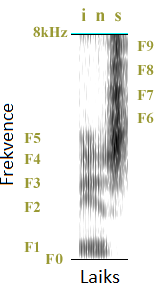
\includegraphics[width=0.25\textwidth]{wave} 
\caption{Spektogramma \cite{DynamicTimeWrapping}}  \label{formantas2} 
\end{figure}

 Pirmās formantas frekvenci parasti nosaka pēc mēles augstumu izrunājot skaņas. Otrās formantas frekvenci nosaka, tas cik tālu mēle ir uz priekšu vai atpakaļ \cite{edist}.
 
Augstie priekšējie patskaņi veidojas kad mēle tiek virzīta uz aukslējām un uz priekšu tuvojoties augšējai lūpai.

Zemie priekšējie patskaņi veidojas kad mēle ir zemu un uz priekšu tuvojoties apakšējai lūpai.

Augstie aizmugurējie patskaņi veidojas kad mēle tiek virzīta uz aukslējām un tai pašā laikā 
mēle tiecas uz rīkles aizmuguri. 

Zemie aizmugurējie patskaņi veidojas kad mēle ir zemu un tiecas uz  rīkles aizmuguri\cite{dtw49}.

 Jo formanta $F_2$ ir augstāka jo vairāk uz priekšu ir mēle, bet jo formanta $F_2$ ir zemāka jo vairāk uz atpakaļu ir mēle.
 
 Jo formanta $F_1$ ir augstāka jo tuvāk mēle ir pie aukslējām , bet jo formanta $F_2$ ir zema jo zemāk ir mēle un atvērtāks žoklis \cite{dtw50}.

Attēlā \ref{formantas3} bildē pa labi var redzēt, kuras $F_1$ un $F_2$ raksturo angļu valodas patskaņus 'a', 'i', 'u' un kā arī šo patskaņu novietojumu un mēles pozīciju izrunājot šos patskaņus.

\begin{figure}[H] \centering
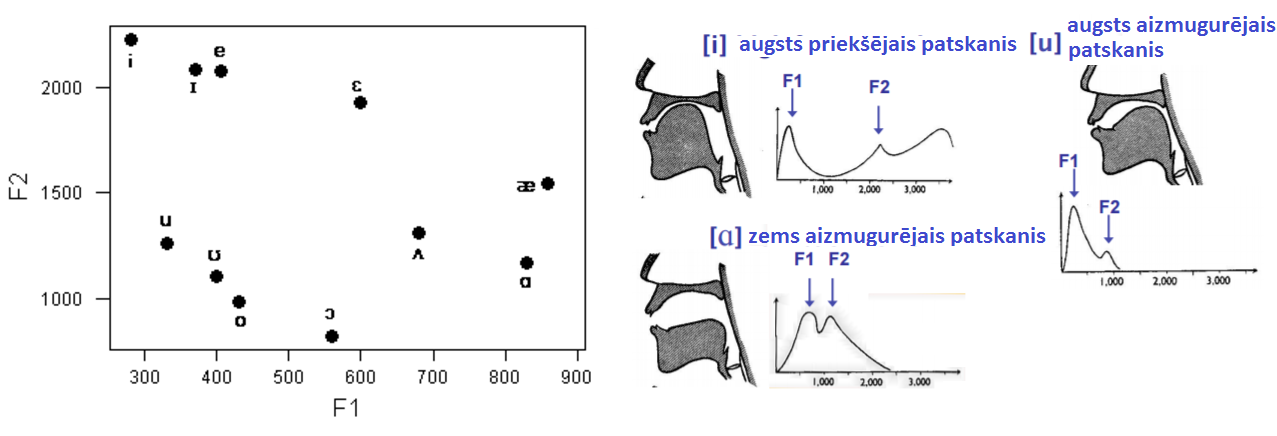
\includegraphics[width=1.00\textwidth]{vowels2} 
\caption{Patskaņa $F_1$ pa horizontālo un $F_2$ pa vertikālo asi (pa kreisi), mēles pozīciju izrunājot patskaņus 'a','u','i' un to formantu $F_1$, $F_2$ grafisks attēlojums(pa labi)
) \cite{edist}, \cite{http://www.charlesames.net/pdf/JamesKirby/lecture12-hanoi-4up.pdf}}  \label{formantas3} 
\end{figure}


\section{Patskaņu modelēšana}
\label{appendix:makevowel}
Darbā tiek izmantota Audiotoolbox \cite{dtw38} metode MakeVowel. Šī metode ir paredzēta vienkāršu patskaņu izveidei. Metodes izsaukšanas sintakse ir :
\begin{lstlisting}
y=MakeVowel(len,pitch,sampleRate, f1,f2,f3)
\end{lstlisting}

, kur

$len$ - signāla garums, 

$pitch$ - signāla augstums. Augstuma mainīgie var būt vai nu skalārs lielums, kas norāda faktisko augstuma frekvenci vai arī impulsu vietu masīvu. Izmantojot impulsu masīvu var izveidot patskaņus ar dažādiem augstumiem. Impulsu masīvu var izveidot izmantojot Audiotoolbox metodi FMPoints, ar kuru detalizētāk var iepazīties avotā \cite{dtw17}. 

$sampleRate$ - patskaņa izgūšanas frekvence,

$f1,f2,f3$ - Formantu frekvences. Formantu frekvenču vietā var norādīt, piemēram, patskaņus 'a', 'i', 'u', kuru formantas jau pēc noklusējuma ir norādītas metodē un veidojot patskaņus formantas tiek automātiski izvēlētas \cite{dtw17}.
\begin{lstlisting}
vowel=MakeVowel(1000,FMPoints(Len,randi([50,500],1,1)),16000,'a')
\end{lstlisting}

Pēc tam izveidotajam signālam uzliek Gausa balto troksni.

\begin{lstlisting} 
vowel = awgn(vowel,30,'measured'); 
\end{lstlisting}

Tiek iegūts hamming logs.

\begin{lstlisting}
w = hamming(Len)
\end{lstlisting}

, kur 

Len - signāla garums,

Hamming - MATLAB iebūvētā funkcija, kas izveido hamming logu, par hamming logu ir aprakstīts tālāk darbā.

Beigās signāls tiek reizināts ar hamming logu. 

\begin{lstlisting}
vowel = vowel.*w'
\end{lstlisting}


\chapter{Skaņas signāla īpašību izgūšana}

Lai iegūtu precīzākus rezultātus runas atpazīšanā, nav nepieciešams izmantot visu informāciju, ko satur skaņas signāls. Nepieciešams izgūt īpašības, kas raksturo skaņas signālu un izmantojot šīs īpašības var precīzāk salīdzināt dotos skaņas signālus. Īpašību izgūšanas pamatā ir nevajadzīgās informācijas atmešana, tādējādi atvieglojot klasifikatora apmācību koncentrējoties uz derīgajām signāla īpašībām. Darbā tiek izmantotas trīs veida īpašības MFCC, LPCC, RASTA-PLP, kas tiks aprakstītas tālāk \cite{knn}.
\section{Logošana}
Logošana nozīmē, ka signāls tiek reizināts ar logu. Rezultātā tiek pieņemtas nulles vērtības visur, izņemot konkrētā skaņas signāla intervālā, kuru tiek ņemti paraugi ar noteiktu amplitūdu, ko nosaka logs. Ja pieņem, ka signāls ir bezgalīgs, var atmest visas nulles un atstāt tikai datus, kas tiks izmantoti apstrādei un analīzei.
Viens no logiem ir taisnstūra logs savas formas dēļ, ko var redzēt attēlā \ref{windows}. Viena no problēmām ar šāda veida logu ir pēkšņa maiņa pie stūriem, kas rada tā saucamo stūra efektu un tas var radīt signāla kropļojums. Lai samazinātu signāla kropļojumu parasti izmanto Hamming logu, tāpēc, ka šis logs pieņem nulles vērtības galos un pakāpeniski aiziet līdz vērtībai, tādējādi signāla stūri netiek uzsvērti samazinot stūru efektu \cite{Windowing}.
Attēlā \ref{cadrs} var apskatīt, kā tiek paņemts konkrēts kadrs no signāla, tam pielietota logošana un tad tiek ņemts nākošais kadrs, kuram tiek veikts tas pats, kas iepriekšējam kadram.

\begin{figure}[h] \centering
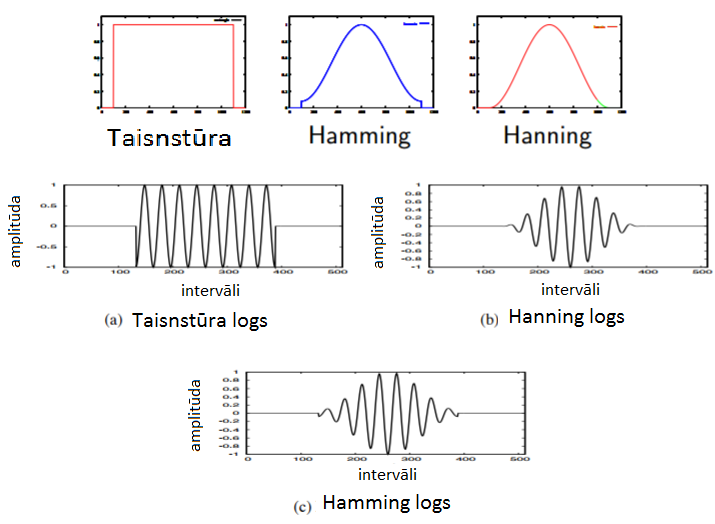
\includegraphics[width=0.70\textwidth]{humming} 
\caption{Taisnstūra logs (pa kreisi), taisnstūra loga skaņas viļņa forma (zem taisnstūra loga), Hamming logs (pa vidu), Hamming loga skaņas viļņa forma(apakšā), Hanning logs(pa labi),Hanning loga skaņas viļņa forma (Zem Hanning loga \cite{dtw9}}  \label{windows} 
\end{figure}

\section{Mel Frekvences Cepstrālie koeficienti}
Mel Frekvences Cepstrālie koeficienti ir īpašības, kas ir plaši izmantotas automātiskā runas atpazīšanā, lai salīdzinātu skaņas signālus. Šos koeficientus pirmo reiz prezentēja 1980. gādā un vēl aizvien mūsdienās tie tiek plaši izmantoti. 
Mel skala tika izveidota eksperimentam nolūkos, kur tika pētīts, kā cilvēka auss interpretē frekvences. Tas notika 1940 gadā. Šī eksperimenta mērķis bija parādīt cilvēka skaņas uztveres sistēmu lineārā skalā. Tika veikti secinājumi, ka frekvences tiek lineāri uztvertas no 0-1000Hz, bet pēc tam skala paliek logaritmiska \cite{http://practicalcryptography.com/miscellaneous/machine-learning/guide-mel-frequency-cepstral-coefficients-mfccs/}.
Kā iegūt MFCC tiek attēlots shēmā \ref{mfcc} un tālāk pa punktiem tiek apskatīts katrs solis.

\begin{figure}[h] \centering
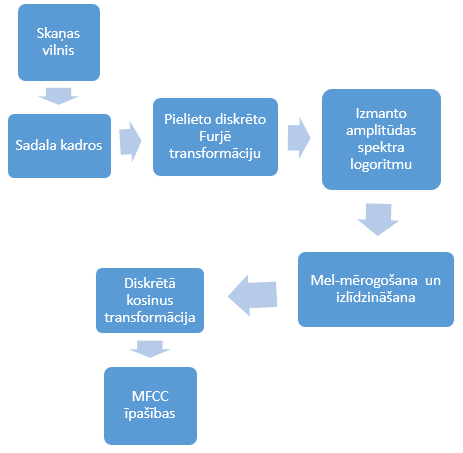
\includegraphics[width=0.90\textwidth]{mfcc} 
\caption{Mel Frekvences Cepstrālo Koeficientu iegūšanas algoritma diagramma \cite{dtw12}}  \label{mfcc} 
\end{figure}

\begin{enumerate}
\item Sadala skaņas signālu kadros \ref{cadrs} un pielietojot logošanas funkciju, parasti Hamming logu, lai noņemtu stūru efektu noteiktā intervālā. \begin{equation}
s(n)\times w(n),
\end{equation}

kur 

s(n) ir signāla kadrs,

w(n) ir nodefinēts kā Humming logu, kuru aprēķina pēc vienādojuma:

\begin{equation}
w(n, \alpha) = (1 - \alpha) - \alpha cos(2\pi \frac{n}{(N-1)}) ,0\leq n \leq N-1,
\end{equation}

kur 

N - kopējo skaņas intervālu skaitu,

n - ir mainīagis kas pieņem vērtības $0\leq n \leq N-1$ \cite{dtw48}. 

Dažādas $\alpha$ vērtības atbilst dažādām līknēm ar Haminga logiem \ref{humlin}.
 \begin{figure}[h] \centering
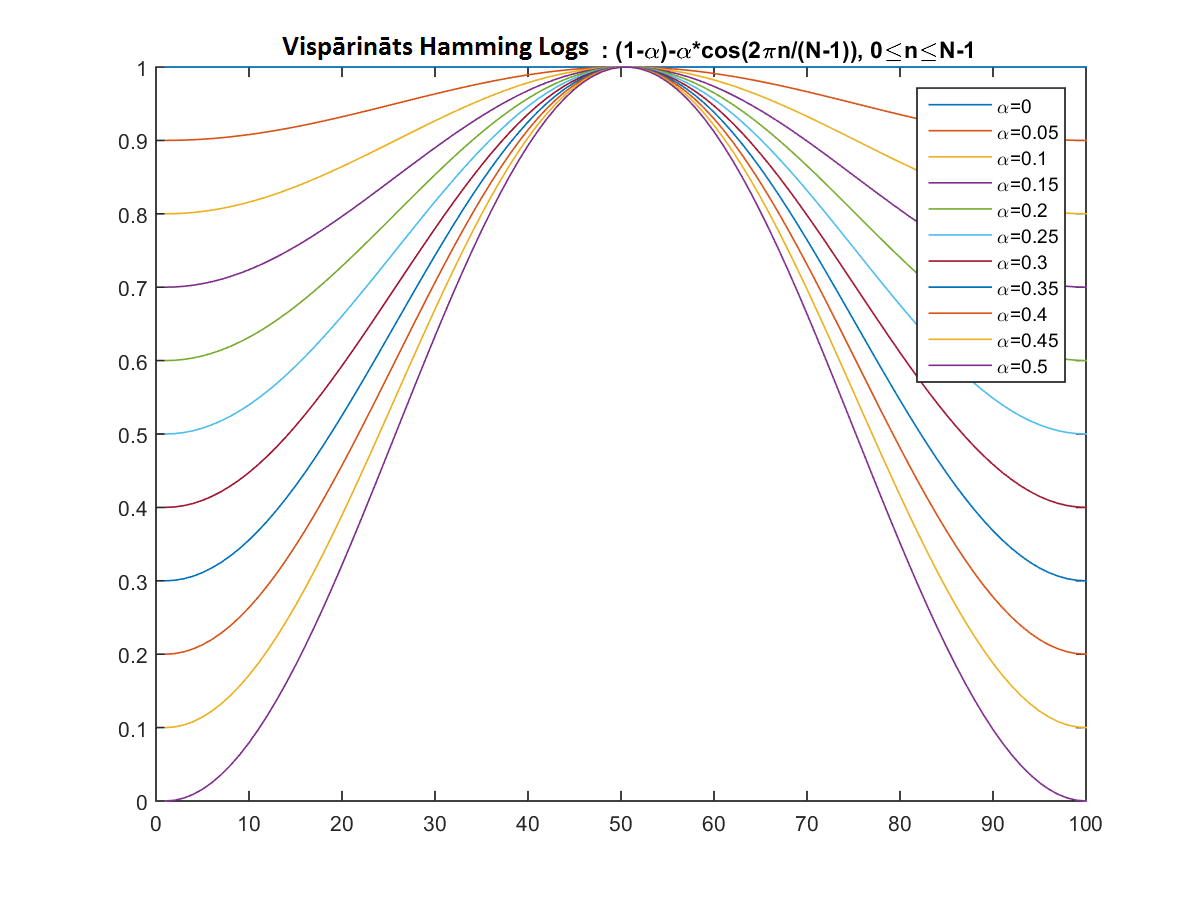
\includegraphics[width=1.00\textwidth]{hamming} 
\caption{Vispārināts Hamming logs ar dažādām $\alpha$ vērtībām \cite{MFCC}}  \label{humlin} 
\end{figure}

 \begin{figure}[H] \centering
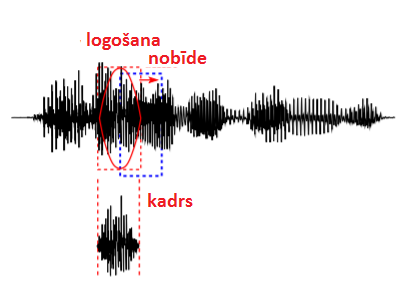
\includegraphics[width=0.70\textwidth]{framing0} 
\caption{Signāla kadru logošana \cite{dtw9}}  \label{cadrs} 
\end{figure}


Mērķis ir radītas nelielas (20ms) signāla daļas, kas ir īslaicīgi stacionāras. Katram kadram tiek ģenerēts cepstrālo īpašību vektors.
\item Katram kadram pielieto diskrēto Furjē transformāciju par, kuru detalizētāk var uzzināt avotā \cite{diskrete}. Saglabā tikai logaritmu no amplitūdu spektra un atmetam informāciju par fāzi. Tiek izmantots amplitūdas spektra logaritms, jo uztvertā signāla skaļums ir apmēram logaritmisks. 
\item Nepieciešams nolīdzināt spektru un jāizceļ svarīgākās frekvences. Šo procesu var apskatīt attēlā \ref{minimize-freq}. Zemākās frekvences runā ir daudz svarīgākas nekā augstās frekvences, tāpēc, lai nolīdzinātu spektru pielieto ‘Mel’ frekvenču skalu. Mel skala ir logaritmiska skala, kas attēlo to, kā cilvēka auss
uztver skaņu. 

  \begin{figure}[H] \centering
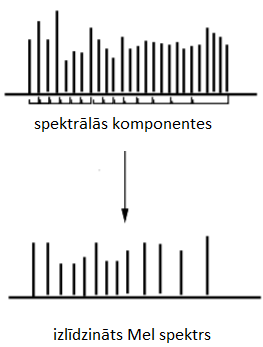
\includegraphics[width=0.30\textwidth]{dsf} 
\caption{Signāls frekvenču telpā (augšā) un signāls, kam veikta frekvenču izlīdzināšana \cite{dtw12}}  \label{minimize-freq} 
\end{figure}
Mel funkciju 

\begin{equation}
mel(f)=2595 \times ln(1+\frac{f}{700}),
\end{equation}

kur 

f - frekvence,

var apskatīt attēlā \ref{mel}, kur var redzēt, ka funkcija ir apmēram lineāra zem 1kHz un pēc tam kļūst logaritmiska.

 \begin{figure}[H] \centering
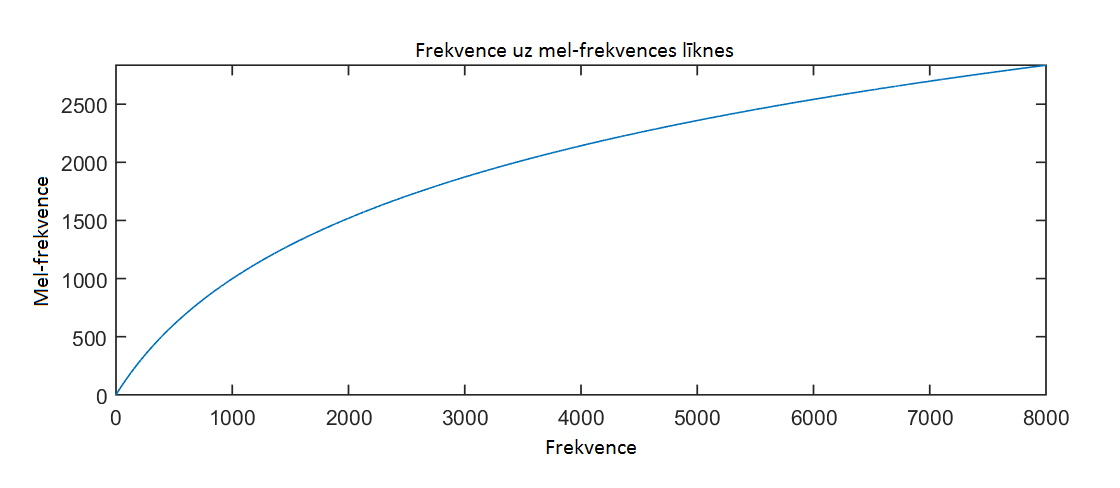
\includegraphics[width=1.00\textwidth]{mel} 
\caption{Mel skalas grafiks \cite{MFCC}}  \label{mel} 
\end{figure}


\item Mel-spektra komponentes, kas tiek aprēķinātas katram kadram ir augsti korelētas, tāpēc kā pēdējo darbību ir nepieciešams veikt kadru transformāciju Mel-spektrālajiem vektoriem, kas dekorelē to komponentes. Lai to izdarītu izmanto Diskrēto Kosinusa transformāciju \cite{dtw25} un tad katram kadram tiek iegūtas apmēram 13 cepstrālās īpašības \cite{MFCC}, \cite{http://citeseerx.ist.psu.edu/viewdoc/download?doi=10.1.1.800.1305&rep=rep1&type=pdf}. 


\end{enumerate}
\section{Lineārās Prognozēšanas Cepstrālie Koeficienti }

LPCC iegūšanas algoritmu var apskatīt attēlā \ref{lpcc}. 
 \begin{figure}[H] \centering
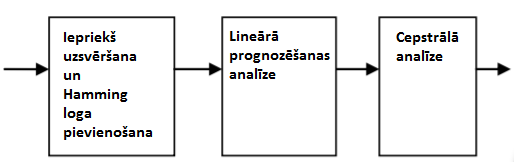
\includegraphics[width=1.00\textwidth]{lpcc} 
\caption{ Linear Prognozēšanas Cepstrālo koeficientu iegūšanas diagramma  \cite{http://citeseerx.ist.psu.edu/viewdoc/download?doi=10.1.1.800.1305&rep=rep1&type=pdf}}  \label{lpcc} 
\end{figure}

Tiek veikta ievadītā signāla priekšapstrāde izmantojot pirmās kārtas augstfrekvenču filtru. To veic, jo skaņas signālā vairāk ir izplatītas zemās frekvences nekā augstās frekvences un ir nepieciešams palielināt augsto frekvenču enerģiju. 

 Tālāk signāls tiek sadalīts kadros. Lai mazinātu pārtrauktību katra kadra beigās veic logošanu izmantojot Hamming logu:
\begin{equation}
w(n) = 0.54 – 0.46cos(2\pi \frac{n}{N}); 0 \leq n \leq N,
\end{equation}
kur 

N ir logošanas funkcijas garums jeb kopējo skaņas intervālu skaits,

n - ir mainīgais kas pieņem vērtības $0\leq n \leq N-1$ \cite{dtw48}. 

Lineārā prognozēšanas analīze ir balstīta uz hipotēzes, ka vokālā trakta forma nosaka skaņas rakstura īpašības. Digitāls visu-polu filtrs \cite{allpole} tiek pielietots lai modelētu vokālo traktu un šim filtram eksistē pārveidošanas funkcija reprezentēta z telpā 
\begin{equation}
V(z)=\frac{G}{1-\sum\limits_{k=1}^pa_kz^{-k}},
\end{equation}


kur 

V(z) – vokālā trakta pārveidošanas funkcija, 

G – pastiprinājums no filtra, 

$a_k$ ir kopa no audio regresijas koeficientiem (LPC),

p – visu-polu filtru kārtība. 

Lai noteiktu LPC un pastiprinājumu no filtra izmanto Auto korelāciju. 

Pēdējais solis, kas jāveic ir cepstrum analīze. Ir divi veidi kā to izdarīt – FFT cepstrum \cite{fft} un LPC cepstrum \cite{lpcc}. No LPC iegūst cepstrālos koeficientus veicot rekursīvas procedūras un beigās tiek iegūti koeficienti ko sauc par LPCC \cite{http://citeseerx.ist.psu.edu/viewdoc/download?doi=10.1.1.800.1305&rep=rep1&type=pdf}. 



\section{Relatīvā Spektrālā Transformācija-Uztveres Lineārā Prognozēšana}
 

MFCC ir populārākais runas īpašību reprezentācijas veids. Bet vēl eksistē arī runas īpašību reprezentācijas veids kā RASTA-PLP jeb 
Relatīvā Spektrālā Transformācija-Uztveres Lineārā Prognozēšana. 
PLP sākotnēji ierosināja Hynek Hermansky, kā veidu, lai deformētu spektru, lai
minimizētu atšķirību starp skaļruņiem vienlaikus saglabājot svarīgu balss informāciju \cite{H2}.
RASTA ir atsevišķa metode, kas pielieto joslu caurlaides filtru katrai frekvenču
apakšjoslas enerģijai \cite{H1}.
Kopumā RASTA filtrs ir joslu caurlaides filtrs. Tā mērķis ir apspiest lēnas un ātrās kanāla variācijas. Vairāk par RASTA filtru tiek aprakstīts avotā \cite{H1}.

Līdzīgi kā LPCC tiek veikta signāla priekšapstrāde un pēc tam signāls tiek sadalīts kadros un pielietota logošana, lai noņemtu stūra efektu.



RASTA-PLP kā viena no darbībām tiek veikta frekvenču deformāciju uz Bark skalu. Vispirms, lai to izdarītu nepieciešams
pārveidot frekvences uz bark, kas labāk ataino cilvēka dzirdes frekvenču izšķirtspēju.
Par Bark skalu detalizētāk ir aprakstīts avotā \cite{https://ccrma.stanford.edu/courses/120-fall-2003/lecture-5.html}.  

%Vienlīdzīga skaļuma iepriekš uzsvēršana ir nepieciešama, lai kompensētu ne vienmērīgo skaļuma uztveri pie dažādām
%frekvencēm. Skaļuma iepriekš uzsvēršana funkciju var apskatīt avotā \cite{dtw50}

Izlīdzinātās vērtības tiek pārveidotas balstoties uz Stīvena skaļuma enerģijas intensitātes likuma, kas ir detalizētāki aprakstīts avotā \cite{http://acousticslab.org/psychoacoustics/PMFiles/Module04.htm}. 

Ar RASTA-PLP koeficientu iegūšanas shēmu var iepazīties detalizētāk un par to, kas notiek katrā etapā avotā \cite{http://www.icsi.berkeley.edu/pubs/techreports/tr-91-069.pdf}.



\section{Signālu atšķirības novērtējums}
Kad esam izguvuši signāla īpašības var sākt salīdzināt skaņas signālus. Divu skaņas signālu salīdzināšanai tiek izmantotas distances. Jo mazāka vērtība starp diviem signāliem, jo līdzīgāki tie ir. Darbā tiek izmantotas Eiklīda un  Bhattacharyya distances. 
Eiklīda distance \cite{eucl}:
\begin{equation} \label{eq:1}
\sqrt{\sum\limits_{i=1}^n (p_{i} - q_{i})^2},
\end{equation}
kur
$n$ - elementu skaits,
$p_i$ -Pirmā vektora  i-tais elements,
$q_i$ - Otrā vektora i-tais elemets.
 

Bhattacharyya distances, kuru oriģināli lieto histogrammu atšķirības aprēķināšanai attēlu apstrādē \cite{https://pdfs.semanticscholar.org/75d0/f2a4a2dff5cce4eb4097c2e68e1ff75ae569.pdf}:
\begin{equation}
d(H_1,H_2) = \sqrt{1-\frac{1}{\sqrt{\overline{H}_1\overline{H}_2N^2}}\sum\limits_{I}\sqrt{H_1(I) \times H_2(I)}},
\end{equation}
kur

$H_1$ - pirmā histogramma,

$H_2$ - otrā histogramma,

$N$ - kopējais histogrammas elementu (grozu) skaits. 
 



\chapter{Klasifikātori}
\section{Klasifikācija}
Klasifikācijas uzdevums ir noteikt nezināma elementa piederību, kādai noteiktai klasei. Nepieciešams vispirms izveidot klasifikācijas modeli izmantojot vienu no algoritmiem -  lēmuma koka klasifikators, uz noteikumiem balstīti klasifikatori, neironu tīkli, atbalsta vektor mašīnas un naivais Bayes klasifikators \cite{http://www.sciencedirect.com/science/article/pii/S0957417410011759}. 
Lai klasifikators pildītu tam paredzētās funkcijas ir nepieciešams veikt klasifikatorā apmācību. Klasifikatoram padodot kopu ar apmācības datiem pēc kuriem tas apmācās. Dati jau ir sadalīti pa attiecīgajām klasēm. Dati var būt gan jēldati (raw), gan arī izgūtas raksturojošas īpašības (features), kas ir daudz efektīgāks datu veids klasifikatora apmācībai. No šiem datiem lielā mērā ir atkarīga klasifikācijas modeļa efektivitāte. 
Kad klasifikators ir apmācīts var veikt testa datu klasifikāciju izmantojot attiecīgo algoritmu. 
Darbā tiek apskatīti daži no populārākajiem algoritmiem, kurus pielieto, lai klasificētu testa datus \cite{knn}. 

\section{K-tuvāko kaimiņu klasifikators}


KNN klasifikatora būtība ir piešķirt nezināmajam īpašību vektoram x nosaukumu attēlā \ref{klass} , balsoties uz datiem no viena no iepriekš apmācītajiem īpašību vektoriem, kas atrodas x vektoram vistuvāk telpā ko sauc par īpašību telpu  (no angļu val. feature space). Tiek izmantota apmācības datu kopa, kuru apzīmē ar T, lai identificētu x piederību kādai no iespējamajām klasēm. Vispirms tiek noteiktas vidējās un maksimālās vērtības vektoriem, kas atrodas kopā T. Tad tiek atrastas vidējās vērtības un maksimālās vērtības nezināmajam vektoram x. Pēc tam īpašību telpā tiek aprēķināta distance no x līdz citiem vektoriem, lai noteiktu kuri k vektori T kopā atrodas vistuvāk x. Ja lielākā daļa tuvāko k elementu satur līdzīgas maksimālās un vidējās vērtības kā vektors x tad elements x tiek klasificēts attiecīgi. 


 \begin{figure}[H] \centering
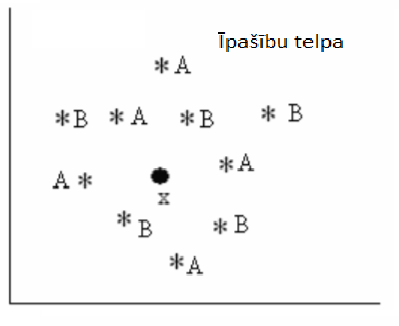
\includegraphics[width=0.40\textwidth]{knn} 
\caption{Īpašību plakne ar divu klašu elementiem (A un B) un vienu nezināmo elementu x \cite{knn}}  \label{klass} 
\end{figure}

KNN klasifikatoram pastāv divas problēmas.
\begin{enumerate}

\item	Ir nepieciešams atrast piemērotu distances algoritmu, kas varētu precīzāk noteikt, kuri k elementi ir vistuvāk elementam x. 
Dažas no distancēm kuras var izmantot ir
\begin{itemize}
\item	 Eiklīda distance, kas bija iepriekš aprakstīta sadaļā \ref{eq:1}.


\item	City-block distance
\begin{equation}
D_{city-block}(x,y)=\sum\limits_{i=1}^n |x_{i} - y_{i}|,
\end{equation}

kur

$n$ - elementu skaits,

$x_i$ -Pirmā vektora  i-tais elements,

$y_i$ - Otrā vektora i-tais elements.

\end{itemize}

\item	K elementu izvēle. Ja izvēlas lielu k vērtību tad iegūst lineāru klasifikatoru, kas piešķir vērtību x balstoties uz to, kuras klases elementi ir visvairāk, piemēram, ja $k =7$, tad ir 4 A elementi un 3 B elementi tad x tiek piešķirta A vērtība ievērojot vairākuma balsošanas noteikumu, kaut arī jāņem vērā, ka elements x atrodas vistuvāk 3 B elementiem. Atrastu optimālo k vērtību vienmēr ir problēma \cite{knn}.  
\end{enumerate}

\section{Lēmuma koka klasifikators}
DT klasifikatora būtība ir koka struktūras izveide, kur mezgli ir doto datu atribūtu vārdi, zari ir atribūtu vērtības, bet lapu mezgli ir klašu nosaukumi. Struktūru var apskatīt attēlā \ref{decidion-tree}.
 \begin{figure}[H] \centering
\begin{forest} 
for tree={
  grow=east,
  draw=cyan,
  circle,
  line width=0.3pt,
  parent anchor=east,
  child anchor=west,
  edge={draw=cyan},
  edge label={\Huge\color{black}},
  edge path={
    \noexpand\path[\forestoption{edge}]
      (!u.parent anchor) -- ([xshift=-1.6cm].child anchor) --    
      (.child anchor)\forestoption{edge label};
  },
  l sep=2cm,
} 
[Sakne,rectangle, s sep=35pt,
  [Kopa1,edge label={node[Below]{Zars}}
  [Klase,edge label={node[Below]{Zars}}
    ]
    [Klase,edge label={node[Above]{Zars}}
    ]
  ]
  [Kopa2,edge label={node[Above]{Zars}}
    [Klase,edge label={node[Below]{Zars}}
    ]
    [Klase,edge label={node[Above]{Zars}}
    ]
  ]
]
\end{forest}

\caption{Lēmuma koka struktūras}  \label{decidion-tree} 
\end{figure}

 
Lai izveidotu lēmuma koku nepieciešams veikt trīs soļus \cite{dtw14}:
\begin{enumerate}

\item	Izvēlēties īpašību pēc, kuras tiek sadalīti esošie dati

\item	Sadalīt dotos datus datu kopās, ņemot vērā kritēriju, kas ir izvēlētā īpašība.

\item	Nepieciešams atkārtot augšējās darbības līdz tiek atrasti lapu mezgli visos zaros. 

\end{enumerate}
Problēma klasifikatorā ir tas ka var notikt pārmācīšanās, ja klasificējot testa datus iegūstam ļoti sliktu precizitāti vai arī kad kokam ir pārāk daudz zaru, kas ataino anomālijas, kas radušās trokšņa vai netipisku datu rezultātā.
Lai optimizētu koku ir nepieciešams atmest tos zarus, kas nav noderīgi priekš klasifikācijas 

\begin{enumerate}

\item	Viena no metodēm ir Pirms-Atzarošanās jeb puse no koka tiek izveidota agri. Tas nozīmē, ka nedrīkst sadalīt tos mezglus, kuru vērtības ir zem noteiktās atmetamo vērtību robežas. Problēma ir, ka ir grūti noteikt šo vērtību atmešanas robežu.

\item	Post-Atzarošanās jeb atmest zarus no pabeigta koka. Tas nozīmē, ka nepieciešams iegūt pakāpeniski atzarotu koka secību. Tam nepieciešams izmantot atsevišķu datu kopu no apmācīšanas datiem, lai varētu izlemt, kurš ir labākais atzarotais koks. 
Kad klasificējam, nepieciešams nodrošināt to, ka dati būs pēc iespējas tīrāki \cite{dtw14}. 

\end{enumerate}


\section{Atbalsta vektora mašīna}

SVM veic klasifikācijas uzdevumus veidojot hiper plakni daudzdimensionālā telpā, kas atdala dažādu klašu nosaukumus \cite{http://users.ecs.soton.ac.uk/srg/publications/pdf/SVM.pdf}. Tā sakot SVM ir balstīts uz konceptu, ka eksistē lēmuma plaknes, kas nosaka lēmuma robežas. Lēmuma plakne ir tā, kas atdala objektu kopas, kas pieder atsevišķām klasēm. SVM koncepts tiek attēlots attēlos \ref{svm1},\ref{svm2},\ref{svm3}. Attēlā \ref{svm1} ir attēlots lineārs klasifikators, kas atdala elementus izmantojot līniju. Attēlā \ref{svm2} ir attēlota daudz sarežģītāka struktūra, kad nepieciešams veikt optimālu atdalīšanu. Attēlā \ref{svm3} tiek attēlota SVM ideja. Ir nepieciešams veikt objektu transformāciju no vienas telpas otrā, lai atrastu optimālu līniju, kas veido lineāru klasifikatoru, atdalot vienas klases objektus no otras klases objektiem izmantojot matemātiskas funkcijas, kuras sauc par kodolu (no angļu val. kernel). 


 \begin{figure}[H] \centering
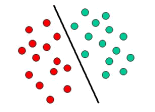
\includegraphics[width=0.40\textwidth]{SVMIntro1} 
\caption{Divas klases, kas atdalītas ar lēmuma robežu \cite{http://www.statsoft.com/Textbook/Support-Vector-Machines}}  \label{svm1} 
\end{figure}

 
  \begin{figure}[H] \centering
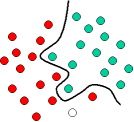
\includegraphics[width=0.40\textwidth]{SVMIntro2} 
\caption{Divas klases, kas atdalītas ar nelineāru lēmuma robežu \cite{http://www.statsoft.com/Textbook/Support-Vector-Machines}}  \label{svm2} 
\end{figure}

 
  \begin{figure}[H] \centering
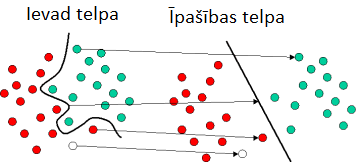
\includegraphics[width=0.70\textwidth]{SVMIntro3} 
\caption{Klašu pārnešana no ievadtelpas uz īpašību telpu \cite{http://www.statsoft.com/Textbook/Support-Vector-Machines}}  \label{svm3} 
\end{figure}

Lai izveidotu šādu hiper plakni SVM izmanto dažādus apmācības algoritmus, kurus izmanto lai minimizētu kļūdas funkciju. Balstoties uz kļūdas funkcijas formu SVM iedalās\cite{http://www.statsoft.com/Textbook/Support-Vector-Machines}:
\begin{enumerate}
\item	Pirmais tips minimizē kļūdas funkciju 
\begin{equation}
\frac{1}{2}w^T w+C\sum\limits_{i=1}^N \xi_i
\end{equation}
 ievērojot ierobežojumus  $y_i(w^T \phi(x_i)+b)\geq 1 - \xi_i $ un $\xi_i\geq0,i=1,...,N $,

 kur 

C ir kapacitātes konstante, 

w ir koeficientu vektors, 

b ir konstante,

$\xi_i$ reprezentē parametrus, lai tiktu gala ar neatdalāmiem ievaddatiem,

indekss i apzīmē N mācību gadījumus,

y reprezentē klašu nosaukumus, 

$x_i$ reprezentē neatkarīgos mainīgos,

kernel funkcija $\phi$ tiek izmantots lai pārveidotu ievaddatus uz īpašību telpu.

Jābūt uzmanīgiem ar C izvēli, jo C ir lielāks jo lielāka aprēķina kļūda un rada pārmācīšanos \cite{http://www.statsoft.com/Textbook/Support-Vector-Machines}.  


\item	Otrais tips minimizē kļūdas funkciju \cite{dtw47}:
\begin{equation}
\frac{1}{2}w^T w-v\rho+\frac{1}{N}\sum\limits_{i=1}^N \xi_i,  0\leq v \leq 1
\end{equation}
 ar ierobežojumu   $y_i(w^T \phi(x_i)+b)\geq \rho - \xi_i,\xi_i\geq0,i=1,...,N $ un $ \rho \geq 0$


\end{enumerate}

Ir vairākas Kernel funkcijas, kas var tikt izmantotas SVM modelim, kā piemēram, Lineārā, Polinomu, RBF (radiālā pamata funkcija), Sigmoida funkcija. Šo funkciju vienādojumus var detalizētāk apskatīt avotā \cite{dtw47}.


\section{Neironu tīkli}
Mākslīgie neironu tīkli ir informācijas apstrādes sistēma,
kuras darbības princips ir balstīts uz smadzeņu uzbūvi, ko veido savienotu neironu anatomiskā struktūra. Mākslīgajiem neironu tīkliem
piemīt daudz vienkāršas apstrādes vienības,
kas dažādi ir savienotas savā starpā \cite{dtw18}.

Neironu tīklu priekšrocība ir tā, ka tiem ir augsta tolerance pret trokšņainiem datiem un ir arī pietiekami labi apmācīts, lai spēja klasificēt jaunus datus, kas atbilst apmācītajam modelim \cite{neirons}.

Neironi tiek organizēti slāņos - ievades, slēptais
un izvades slānis, ko var redzēt attēlā \ref{neiro}. Slēptais slānis ir saistīts gan ar
ievadslāni, gan ar izvadslāni, bet ievadslānis un izvadslānis ir saistīts tikai ar slēpto slāni \cite{dtw18}.
Ievades slānis nesastāv no pilniem neironiem, bet 
gan no elementu vērtībām, kas tiks padoti, kā ieejas 
dati nākošajam neironu slānim. Nākošais ir slēptais 
slānis un vienā neironu tīklā var būt vairāki 
slēptie slāņi. Pēdējais ir izvades slānis, kur 
katrai klasei tiek norādīts viens mezgls.
Katram no šiem mezgliem 
piešķir svaru un tad attiecīgajam elementam tiek 
piešķirta tā klase, kurai ir 
vislielākais svars \cite{neirons}.



Neironi veic samērā vienkāršu darbību. 
Neironi kļūst aktīvi tajā brīdī kad saņemtā signāla
kopējais daudzums pārsniedz aktivizācijas slieksni,
kuru nosaka izmantojot vienu no aktivizācijas
funkcijām. 
Kad mezgls kļūst aktīvs tas pārraida signālu pa pārraides
kanālu līdz nākošajam neironam. Katrs savienojuma 
punkts darbojas kā filtrs, kas samazina vai palielina
signāla intensitāti atbilstoši pēc savām 
individuālajām īpašībām \cite{dtw18}.
Savienojuma punktiem ir fundamentālā funkcija, kas "sver" (maina koeficientu) pārraidītā signāla 
intensitāti, reizinot tos ar svariem, kuru vērtības ir atkarīgas 
no paša savienojuma \cite{dtw18}. 
\begin{figure}[H] \centering
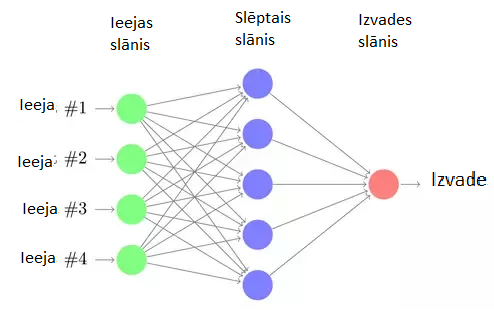
\includegraphics[width=0.80\textwidth]{layers} 
\caption{Neironu tīkla slāņi \cite{layers}}  \label{neiro} 
\end{figure}

\subsection{Mākslīgo neironu tīklu arhitektūra}

Pats svarīgākais ir noteikt kāda būs tīkla arhitektūra
. Cik daudz būs slēpto slāņu un cik daudz neironu 
būs katrā slānī. Ievadslānis tiek noteikts pēc tā
cik daudz būs ievaddatu un izvades slāni nosaka tas, 
cik daudz ir klases. Pats grūtākais ir noteikt no cik daudz slēptajiem slāņiem sastāvēs tīkls. Ja ir par maz slēpto slāņu, grūti izveidot neironu tīkla modeli, kas var veikt sarežģītu ievaddatu atpazīšanu, bet, ja slēpto slāņu ir par daudz, tad var veidoties pārmācīšanās. Par pārmācīšanos tiks aprakstīts sadaļā \ref{appendix:Validation}. Ar diviem slēptajiem slāņiem, parasti 
pietiek, lai varētu izveidot vienmērīgu augsti 
kompleksu datu kopu.
Cik daudz neironu ietvert slēptajā slānī var 
izvēlēties ņemot vērtību starp ievaddatu skaitu 
un izvaddatu skaitu. Bet labāko rezultātus var 
iegūt izmantojot 'trial and error', kur tiek 
izvēlēta koka arhitektūra ar mazāko datu 
šķērss-validācijas kļūdu \cite{layers}. Daudz slāņu tīklos neironus 
izveido tā, lai:
\begin{itemize}

\item Katrs neirons ir savienots ar visiem nākošā slāņa neironiem
\item Starp neironiem, kas pieder vienam slānim nav savienojuma
\item Slāņu skaits un neironu skaits ir atkarīgs no problēmas, kuru nepieciešams atrisināt

\end{itemize}

Daudzslāņu tīklā ir vismaz viens slānis, kas nav savienots ar ievadslāni vai izvadslāni, ko var redzēt attēlā \ref{neiro2} \cite{dtw18}. 

\begin{figure}[H] \centering
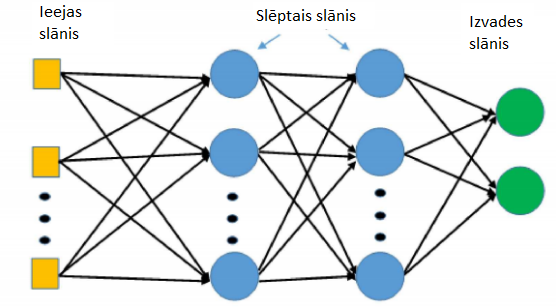
\includegraphics[width=0.70\textwidth]{mnn} 
\caption{Daudzslāņu  tīkla arhitektūra\cite{dtw18}}  \label{neiro2} 
\end{figure}

\subsection{Apmācība}


Tīkla mācību procedūra ir iteratīva. Tas nozīmē, ka tiek nedaudz modificēts
sinaptiskais svars katrā mācīšanās ciklā, ko sauc par epohu, izmantojot 
izvēlētu apmācības datu kopu. Katrā ciklā svaru nepieciešams modificēt, lai samazinātu 
kļūdas funkciju, kas ir specifiska katrai dotajai problēmai. Kad ir veikta apmācība tad var veikt testēšanu izmantojot testa kopu,
lai pārbaudītu tīkla darbību \cite{dtw18}.
\begin{figure}[H] \centering
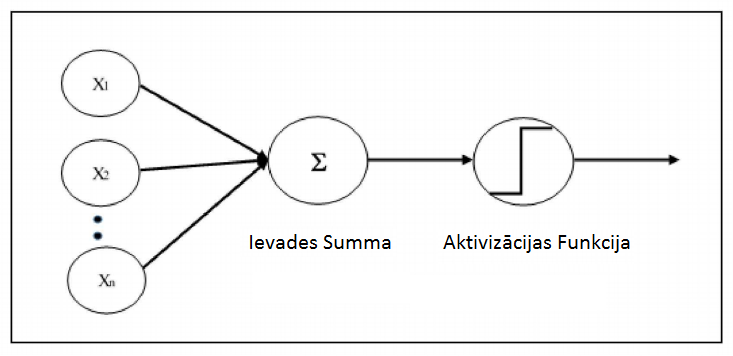
\includegraphics[width=0.80\textwidth]{neiron} 
\caption{Ievadvektora summas aprēķināšana un padošana aktivizācijas funkcijai\cite{dtw18}}  \label{neiro3} 
\end{figure}
Lokālā neirona atmiņa sastāv no svaru vektora $W=(w_1,w_1,...,w_n)$ 
Aprēķins tiek veikts aprēķinot ievades vektora $X=(x_1,x_2,...,x_n)$ summu 
kur katrs elements tiek sareizināts ar attiecīgo svara vektora elementu. Tad 
gala vērtība tiek padota kā ievadvērtība aktivizācijas funkcijai. Šo procesu var redzēt shēmā \ref{neiro3}
Kā aktivizācijas funkciju var izmantot nelineāro sigmoid un citas. Sigmoid ne vienmēr ir labākā. Piemēram, kā aprakstīts šijā avotā: \cite{stackOverflow}


Apmācība notiek tā, ka apmācību sākumā svaru vektors tiek inicializēts ar nejaušām vērtībām.
Katram apmācības datu kopas elementam tiek aprēķināta kļūda, jeb starpība starp 
vēlamo un patieso rezultātu. Šo kļūdu arī izmanto lai modificētu svarus.
Šo procesu atkārto, padodot tīklam nejaušā kārtībā visus apmācības datu kopas elementus 
kamēr kopējā apmācības datu kopas kļūda nebūs mazāka par noteiktu slieksni vai arī kamēr 
nav sasniegts maksimālais iterāciju skaits.

Daudz slāņu tīklu parasti apmāca izmantojot uzraudzīto apmācību, kur  
apmācībai izmanto atpakaļ izplatīšanās algoritmu. Šis algoritms salīdzina
sistēmas izvades vērtības ar vēlamajām vērtībām. Un tad ņemot vērā iegūto 
kļūdu modificē neironu tīkla sinaptiskos svarus, pakāpeniski pielāgojot izvades vērību kopu
un vēlamo vērtību kopu. Svarīgi ir atcerēties, kaut arī nav iespējams zināt slēpto
slāņu vēlamos rezultātus, vienmēr ir iespējams pielietot uzraudzītu apmācīšanās metodi 
atkarībā no kļūdas samazināšanas funkcijas, pielietojot krītošā gradienta metodes \cite{dtw18}.


\subsection{Validācija}
\label{appendix:Validation}
Pēc apmācībām modeļa precizitāti mēra izmantojot atsevišķu elementu kopu 
ko sauc par validācijas kopu \cite{dtw19}. Validācija ir nepieciešama, lai nepieļautu, ka notiek 
pārmācīšanās. Apmācīšanas un validācijas shēma ir attēlota \ref{valid2} Pārmācīšanās notiek gadījumā, kad tīkls tiek pārāk 
labi apmācīts uz apmācības jeb testa datiem. Neironu tīkla modelis apmācās saglabājot netikai apmācības datu rakstura īpašības, bet arī saglabājot dažādus nejaušus trokšņus. 
Tas nozīmē to, ka piemēram kādi nejauši trokšņi tiek 
piefiksēti un uztverti, kā klasifikācijas 
kritērijs, bet uz jaunajiem ievaddatiem šie kritēriji neattiecas un klasifikators nespēj korekti klasificēt jaunos datus. Modelis tiek ierobežots un tā spēja vispārināt datus ir slikta. \cite{dtw20} . 
 
\begin{figure}[H] \centering
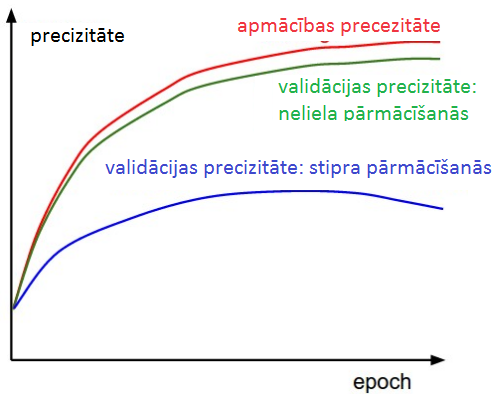
\includegraphics[width=0.60\textwidth]{overfiting} 
\caption{Iespējamie pārmācīšanās varianti \cite{dtw20}}  \label{valid} 
\end{figure}

Grafiks \ref{valid} attēlo iespējamos pārmācīšanās 
variantus modelī. Plaisa starp apmācības 
un validācijas precizitāti norāda uz 
pārmācīšanās apjomu.
Divi iespējamie varianti ir parādīti grafikā. 
Zilā kļūdas validācijas līkne parāda ļoti zemu
apmācības precizitāti un to, ka notiek liela pārmācīšanās.
Redzot šāda veida scenāriju ir nepieciešams vai nu 
palielināt regulāciju vai izmantot vairāk datus.
Zaļā līkne reprezentē to, ka validācijas precizitāte ir samērā 
laba pret apmācības precizitāti. Bet tomēr modeļa enerģija nav pietiekami 
augsta un nepieciešams palielināt modeli palielinot 
parametru skaitu \cite{dtw20}. 

 
\begin{figure}[H] \centering
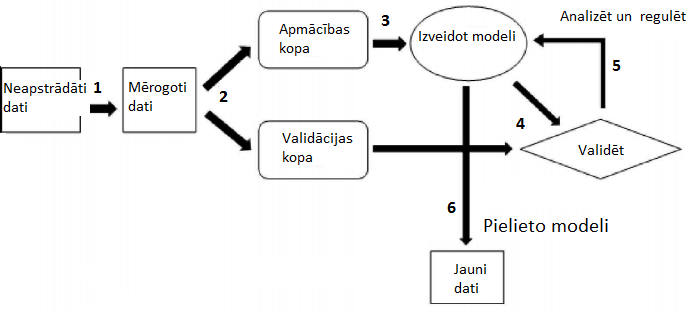
\includegraphics[width=0.90\textwidth]{validation} 
\caption{Tīkla apmācības un validācijas shēma \cite{dtw18}}  \label{valid2} 
\end{figure}

\chapter{Simulācija un rezultāti}

\section{Simulācija izmantojot reālistiskus datus}
 \sloppy
Tika ierakstīti 25 skaņas signāli no 'V','A','Point','Five','C','B', kurus izmantoja klasifikatoru apmācīšanas un testēšanas veikšanai. Klasifikatoru KNN, SVM un DT apmācīšanai izmantoja MFCC un LPCC koeficientus, kurus ieguva no 20 katras klases skaņas signāliem. Testēšanai izmantoja atlikušos piecus skaņas signālus, bet datu nepietiekamības dēļ, klasifikatori nespēja veikt reālistisku skaņas ierakstu klasifikāciju. 

\ref{appendix:piel3} Pielikumā var apskatīt izveidotu MATLAB īpašības koeficientu izgūšanas metodi no reālistiskiem datiem, kā arī klasifikatora, šai gadījumā KNN klasifikatora, apmācīšanas metodi \ref{appendix:piel4} pielikumā un testēšanu metodi \ref{appendix:piel5} pielikumā. 

Kā arī tika ierunāti 4 skaņas signāli no 'Banka','Iela','Upe','I','O','E'. Tika arī ierunāti 7 skaņas signāli no 'Maize', kur četrus skaņas signālus ierunāja viens runātājs, bet pārējos trīs cits runātājs. Šos skaņas signālus izmantoja, lai veiktu salīdzināšanu, līdzīgi kā to darīja A. Šilinis savā bakalaura darbā \cite{Pacienta-runas-kvalitātes-noteikšanas-automatizētas-sistēmas-izstrāde}. Izveidoto skaņas signālu salīdzināšanas metodi var apskatīt \ref{appendix:piel1} pielikumā. 

Skaņas signālus ierunāja izmantojot MATLAB vidē izveidotu skriptu, ko var apskatīt \ref{appendix:piel2} pielikumā.


\section{Simulācija izmantojot ģenerētus datus}

Ņemot vērā klasifikācijas rezultātus ar reālistiskiem datiem, lai veiktu klasifikatoru (Lēmuma koka, K-tuvākā kaimiņa un atbalsta vektor mašīnas) salīdzināšanu pie dažādiem koeficientiem MATLAB vidē tika izveidota funkcija ,kas kā ievaddatus saņem: 
\begin{itemize}
\item Fs – izgūšanas frekvence,
\item Len – skaņas signāla garumu,
\item n – skaņas signālu skaits kurus izmantos klasifikatora apmācīšanā, 
\item m – skaņas signāli uz kuriem tiek testēti apmācītie klasifikatori, 
\item dB1 – Gausa Baltais trokšņa signāla-trokšņa attiecība (SNR) apmācības paraugiem,
\item dB2 – Gausa Baltais trokšņa signāla-trokšņa attiecība testa paraugiem,
\item koeficienti – 
'lpcc' - LPCC pielietojot metodi no avota \cite{dtw39},                 
'mfcc' - MFCC pielietojot metodi no avota \cite{dtw39},              
'rastaplp' - RASTA-PLP \cite{dtw41},
\item klasifikators – 
'knn' - k-tuvākā kaimiņa\cite{dtw42},
'tree' - lēmuma koks\cite{dtw43},
'svm' - atbalsta vektora mašīna\cite{dtw44}.
\end{itemize}
Funkcija atgriež confusion matricu C.
\begin{lstlisting}
function C = vowel_clasification(Fs, Len, n, m, dB1 ,dB2, koeficienti, klasifikators)
\end{lstlisting}
Simulācijas blokshēmu var apskatīt attēlā \ref{blockshema}
Tālāk notiek loga izveidošana. Hamming metode atgriež L punktu simetrisku Hamming logu vektoru w \cite{dtw36}.
\begin{lstlisting}
w = hamming(Len);
\end{lstlisting}
Tiek izveidots vektors, kuru aizpilda ar attiecīgo burtu ASCII vērtībām. Cik daudz vērtības katrai apmācītajai patskaņu klasei izveidot nosaka mainīgais n.

\begin{lstlisting}
labels = [97*ones(n,1);117*ones(n,1);105*ones(n,1);111*ones(n,1);101*ones(n,1)]
\end{lstlisting}



Inicializē tukšu struktūras masīvu 
\begin{lstlisting}
samples = {};
\end{lstlisting}
 

Sākas cikls, kur tiek izveidoti skaņas signāli, kur ii mainās no 1 līdz burtu vektora izmēram: 
\begin{lstlisting}
for ii = 1:length(labels)
\end{lstlisting}



Tiek izmantota metode MakeVowel, kas tika aprakstīta iepriekš \ref{appendix:makevowel}, lai izveidotu skaņas signālu.      
\begin{lstlisting}
wave=MakeVowel(Len,FMPoints(Len,randi([50,500],1,1)),Fs,char(labels(ii)))
\end{lstlisting}



    Pievieno balto Gausa troksni skaņas signāla vektoram $wave$. Mainīgais $dB1$ specificē signāla-trokšņa attiecību uz paraugu un to mēra dB (decibelos). $'measured'$ nozīmē, ka pirms pievienot troksni tiek izmērīta skaņas signāla vektora enerģija  \cite{dtw37}. 
\begin{lstlisting}
    wave = awgn(wave,dB1,'measured')
\end{lstlisting}
    
   
Skaņas signāla vektoru sareizna ar transponētu Hamming loga vektoru 
\begin{lstlisting}
    wave = wave.*w'
\end{lstlisting}


    
Tālāk skaņas signāla vektoru, smapling frekvenci un attiecīgo burtu apkopo struktūrā    
\begin{lstlisting}
    samples{ii}.audio = wave
    samples{ii}.Fs = Fs
    samples{ii}.label = char(labels(ii))
\end{lstlisting}


    
Tiek veikta skaņas signāla īpašību izgūšana izmantojot attiecīgo koeficienta iegūšanas metodi, kuru nosaka mainīgais $koeficienti$ 
\begin{lstlisting}
    if strcmp(koeficienti ,'lpcc')
        ceps = msf_lpcc(wave, Fs,'order',12)
    elseif strcmp(koeficienti ,'mfcc')
        ceps = msf_mfcc(wave, Fs);
    elseif strcmp(koeficienti ,'rastaplp')
   [ceps, freqresp,fb,fbrecon,freqrecon] = rastaplp(wave, Fs, 1, 12);
    end
\end{lstlisting}
   

   
Iegto koeficientu masīvu pievieno struktūrai 
\begin{lstlisting}
    samples{ii}.mfcc = ceps(2:end,:)
end
\end{lstlisting}
    
    
Inicializē masīvu ar sākuma vērtībām 0, kas saturēs katra skaņas signāla izgūto īpašību koeficientu vektoru 
\begin{lstlisting}
TRAIN_DATA = zeros(size(samples{1}.mfcc,1)*size(samples{1}.mfcc,2),size(samples,2))
\end{lstlisting}


Inicializētais masīvs tiek aizpildīts ar attiecīgā skaņas signāla izgūtajiem īpašību koeficientiem:
\begin{lstlisting}
for ii = 1:size(samples,2)
    TRAIN_DATA(:,ii) = samples{ii}.mfcc(:);
end
\end{lstlisting}



Tiek inicializēts vektors, kas nosaka kurai patskaņu klasei pieder attiecīgā skaņas signāla izgūto īpašību koeficientu rinda. Vektors tiek aizpildīts mainot $labels$ ASCII elementu vērtības uz burtiem izmantojot iebūvēto MATLAB funkcijas:
\begin{lstlisting}
groups = cellstr(char(labels))
\end{lstlisting}


Notiek klasifikatoru apmācība izmantojot $TRAIN\_DATA$ matricu un groups vektoru. Klasifikatoru nosaka tas kādu vērtību pieņem mainīgais $klasifikators$.
\begin{lstlisting}
if strcmp (klasifikators, 'knn')
    Mdl3 = fitcknn(TRAIN_DATA',groups);
elseif strcmp (klasifikators,  'tree')
    Mdl4 = fitctree(TRAIN_DATA',groups);
elseif strcmp (klasifikators,  'svm')
    Mdl5 = fitcecoc(TRAIN_DATA',groups);
end
\end{lstlisting}


 
Tiek izveidots vektors, kuru aizpilda ar attiecīgo burtu ASCII vērtībām. Cik daudz vērtības katrai testa patskaņu klasei izveidot nosaka mainīgais m.
\begin{lstlisting}
rlabel = [97*ones(m,1);117*ones(m,1);105*ones(m,1);111*ones(m,1);101*ones(m,1)]
\end{lstlisting}


Vektora elementi tiek samainīti nejaušā secībā.
\begin{lstlisting}
rlabel = rlabel(randperm(length(rlabel)))
\end{lstlisting}


Vektoru, kas saturēs prognozētās skaņas signālu klases aizpilda ar sākuma vērtībām 0 izmantojot MATLAB metodi. 
\begin{lstlisting}
observ_label = zeros(size(rlabel))
\end{lstlisting}

Tālāk kā iepriekš seko patskaņa izveide, Gausa baltā trokšņa iegūšana, Hamming loga pievienošana un konkrēto koeficientu izgūšanas metodes izvēle balstoties uz mainīgā $koeficienti$. 
\begin{lstlisting}
for ii = 1:length(rlabel)
    wave=MakeVowel(Len,FMPoints(Len, randi([50,800],1,1)), Fs, char(rlabel(ii)));
    wave = awgn(wave,dB2,'measured');
    wave = wave.*w';
  
    $if strcmp(koeficienti ,'lpcc')$
        ceps = msf_lpcc(wave, Fs,'order',12);
    elseif strcmp(koeficienti ,'mfcc')
        ceps = msf_mfcc(wave, Fs);
    elseif strcmp(koeficienti ,'rastaplp')
        [ceps, freqresp,fb,fbrecon,freqrecon] = rastaplp(wave, Fs, 1, 12);

    end
\end{lstlisting}



Iegūtajai koeficientu matricai atmet pirmo rindu.
\begin{lstlisting}
 ceps = ceps(2:end,:);
\end{lstlisting}


    Pēc tam, kad iepriekšējās darbības ir izpildītas, balstoties uz mainīgā '$klasifikators$' vērtību, tiek pielietos attiecīgais apmācītais klasifikators, lai noteiktu jaunā skaņas signāla klasi, izmantojot MATLAB iebūvēto funkciju predict.
\begin{lstlisting}
    if strcmp (klasifikators, 'knn')
        label = predict(Mdl3,ceps(:)');
    elseif strcmp (klasifikators,  'tree')
        label = predict(Mdl4,ceps(:)');
    elseif strcmp (klasifikators,  'svm')
        label = predict(Mdl5,ceps(:)'); 
    end
\end{lstlisting}
    
    
Klasifikacijas rezultātus saglabā mainīgajā $label$.    
\begin{lstlisting}
label = label{:}
\end{lstlisting}

Pēc tam saglabā rezultātu $observ\_label$ pārvēršot attiecīgās klases burtu par ciparu, kas ASCII skalā reprezentē konkrēto burtu.
\begin{lstlisting}
    observ_label(ii) = double(label);
end
\end{lstlisting}

Izveido beigās matricu \ref{confusionMatrix}, kura salīdzina iegūto klasifikācijas rezultātu vektoru ar rlabel vektoru, kas satur patiesās skaņas signālu klases. Matricā tiek attēlos elementu skaits kas ir klasificēts pie katras klases. 
\begin{lstlisting}
C = confusionmat(rlabel,observ_label);
end
\end{lstlisting}


 \begin{figure}[H] \centering
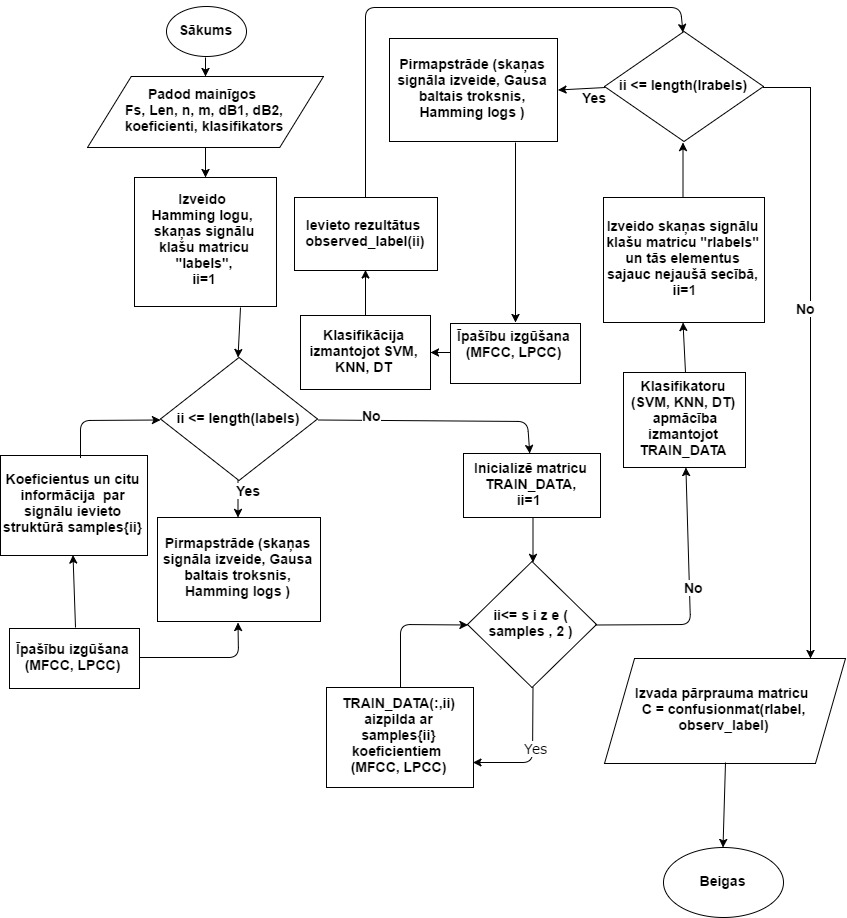
\includegraphics[width=1.00\textwidth]{download} 
\caption{Klasifikatoru apmācīšanas un testēšanas simulācijas shēma}  \label{blockshema} 
\end{figure}

\section{Neironu tīklu                                                                                                                                                   Paternu Atpazīšanas rīks}

\begin{figure}[H] \centering
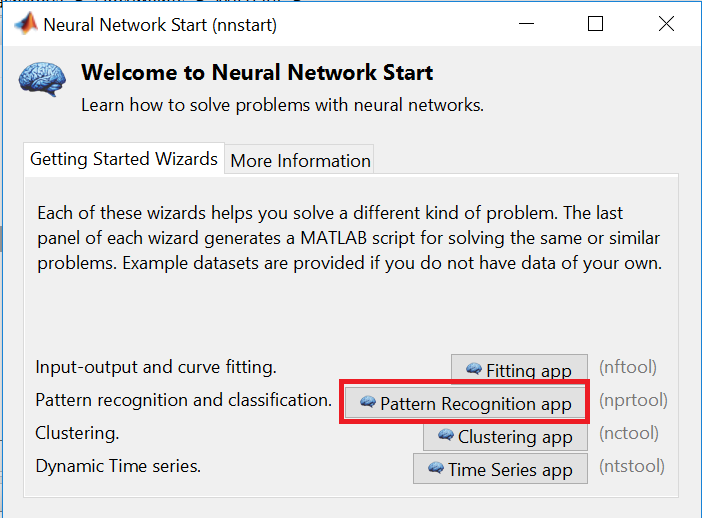
\includegraphics[width=0.60\textwidth]{mat} 
\caption{nnstart. MATLAB Neironu tīklu toolbox. \cite{dtw18}}  \label{mattoolbox} 
\end{figure}

Tiek izmantots MATLAB piedāvātais Neironu tīklu toolbox, kuru var apskatīt attēlā \ref{mattoolbox}, lai veiktu neironu tīklu apmācību, testēšanu un validāciju. No neironu tīklu toolbox izmantot Paternu Atpazīšanas Rīku, kas attēlā \ref{mattoolbox} ir apzīmēts ar sarkanu krāsu. Bet vispirms ir nepieciešams izveidot datu kopu izmantojot izveidotu funkciju MATLAB. 
Funkcijai padod:
\begin{itemize}
\item Fs – izgūšanas frekvence, 
\item Len – skaņas signālu garumu
\item n – elementu skaitu, 
\item dB – Gausa balto trokšņu signāla-trokšņa attiecība,
\item koeficienti -  'LPCC pielietojot metodi no avota \cite{dtw39},                 
'mfcc' - MFCC pielietojot metodi no avota \cite{dtw39},         
'rastaplp' - RASRA-PLP  \cite{dtw41}.
\end{itemize}



Funkcija atgriež skaņas signālu īpašību koeficientu matricu $TRAIN\_DATA$ un matricu
$labels\_target$, kas satur informāciju par to, kurai klasei pieder konkrētā skaņas signāla izgūto īpašību koeficienti. 
\begin{lstlisting}
function [TRAIN_DATA,labels_target ] = vowel_NN_clasification(Fs, Len, n, dB, koeficienti)
\end{lstlisting}

Tālāk kā iepriekš tiek veiktas attiecīgās darbības.
\begin{lstlisting}

w = hamming(Len);

labels = [97*ones(n,1);117*ones(n,1);105*ones(n,1);111*ones(n,1);101 * ones(n,1)];
 
samples = {};

for ii = 1:length(labels)
    wave=MakeVowel(Len,FMPoints(Len, randi([50,500],1,1)), Fs, char(labels(ii)));
    wave = awgn(wave,dB,'measured');
    wave = wave.*w';
    samples{ii}.audio = wave;
    samples{ii}.Fs = Fs;
    samples{ii}.label = char(labels(ii));
    
    if strcmp(koeficienti ,'lpcc')
        ceps = msf_lpcc(wave, Fs,'order',12);
    elseif strcmp(koeficienti ,'mfcc')
        ceps = msf_mfcc(wave, Fs);
    $elseif strcmp(koeficienti ,'rastaplp')

        [ceps, freqresp,fb,fbrecon,freqrecon] = rastaplp(wave, Fs, 1, 12);
    end
    samples{ii}.mfcc = ceps(2:end,:);
end

TRAIN_DATA = zeros(size(samples{1}.mfcc,1)*size(samples{1}.mfcc,2),size( samples ,2));

for ii = 1:size(samples,2)
    TRAIN_DATA(:,ii) = samples{ii}.mfcc(:);
end

\end{lstlisting}


Tiek nodefinēts masīvs, kas saturēs 0, ja skaņas signāls nepieder attiecīgajai klasei un 1, ja pieder klasei. Sākumā inicializē visu masīvu ar 0.

\begin{lstlisting}
labels_target = zeros(length(unique(labels)),size(TRAIN_DATA,2));
\end{lstlisting}


Inicializē mainīgo, kas saturēs vienas klases elementu skaitu ar sākuma vērtību 1.

\begin{lstlisting}
count=1;
\end{lstlisting}

Ciklā label pieņem vērtības no 1 līdz $labels\_target$ matricas pirmās kolonas izmēram.

\begin{lstlisting}
for label= 1:size(labels_target,1)
\end{lstlisting}


    Aizpilda attiecīgos masīva elementus ar vērtībām 1.

\begin{lstlisting}
    labels_target(label,count:count+n-1)=1;
\end{lstlisting}


Palielina $count$ skaitu.

\begin{lstlisting}
    count = count+n;
end
end
\end{lstlisting} 
 


Tālāk, izpildot avotā \cite{dtw40} aprakstītās pamācībās soļus, veic neirona tīklu apmācību, validāciju un testēšanu izmantojot izveidoto datu kopu. Beigās iegūstot pārpratuma matricu \ref{confussion}. 

\begin{table}
\centering
\caption{}
\captionsetup{justification=centering}
\caption*{\textbf{Ģenerēta kļūdas jeb pārpratuma matrica}}
\begin{tabular}{ | l | l | l | l | l |} 
\hline
300 & 0 & 0 & 0 & 0 \\ 
\hline
0 & 289 & 0 & 11 & 0 \\ 
\hline
0 & 0 & 300 & 0 & 0 \\ 
\hline
22 & 3 & 0 & 240 & 35 \\ 
\hline
30 & 0 & 0 & 0 & 270 \\ 
\hline

\end{tabular}
\label{confusionMatrix}
\end{table}

\begin{figure}[H] \centering
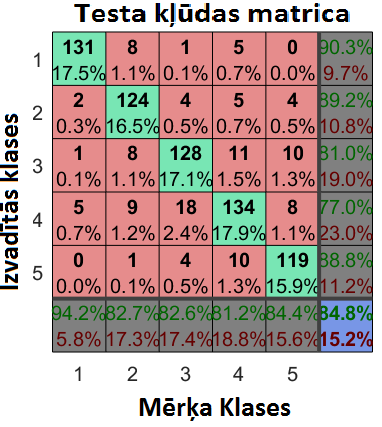
\includegraphics[width=0.45\textwidth]{confussion1} 
\caption{Kļūdas jeb pārpratuma matrica, kur tiek attēlots elementu skaits kas ir klasificēts pie katras klases un pēdējā rindā un kolonā tiek procentuāli aprēķināts cik daudz skaņas signāliem ir noteikta pareizā klase \cite{dtw40}} .  \label{confussion} 
\end{figure}


\section{Rezultāti}

Tiek ģenerēti skaņas signāli ar kopējo garumu 5000 punkti un 16000Hz izgūšanas frekvenci. 
Skaņas signāliem, kurus izmanto apmācībā tiek pievienots Gausa baltais troksnis
ar noteiktu signāla-trokšņa attiecību. Signāliem, kurus izmanto testēšanai, pievieno arī
Gausa balto troksni ar dažādām signāla-trokšņa attiecībām (SNR). 

Tiek ģenerēti 1000 skaņas signāli katrai skaņas signālu klasei, kurus izmanto KNN, SVM, DT klasifikatora apmācībai. Šo klasifikatoru testēšanai tiek ģenerēti 300 testa skaņas signāli. 

Neironu tīklu apmācībai ģenerē 1300 skaņas signālus katrai skaņas signālu klasei. No izveidotās datu kopas 15$\%$ izmanto testēšanai un 15$\%$ izmanto tīkla validācijai.

Signāla īpašību izgūšanai tiek izmantoti MFCC, LPCC koeficienti un uz šiem koeficientiem tik apmācīts KNN, DT, SVM klasifikators
un neironu tīkli. 

Klasifikācija tika veikta izmantojot arī Rasta-PLP koeficientus, bet salīdzinājumā ar rezultātiem, kurus ieguva izmantojot MFCC un LPCC, bija ļoti liela atšķirība starp iegūtajām pārpratuma matricām testējot apmācītos klasifikatorus uz RASTA-PLP koeficientiem. Tā kā RASTA-PLP dažiem klasifikatoriem (KNN, DT, SVM) radīja būtiskas atšķirības veikstpējā, šis koeficientu tips šajā darbā turpmāk netiek apskatīts. 

Rezultātā tiek apkopoti vienā tabulā visu pārpratuma matricu dati pie konkrētas Gausa balto trokšņu signāla-trokšņa attiecības. 

\begin{enumerate}


\item Skaņas signāliem, kurus izmanto apmācībā, tiek pievienots Gausa baltais troksnis
ar 50dB lielu signāla-trokšņa attiecību. Signāliem, kurus izmanto testēšanai, pievieno
Gausa balto troksni ar 50dB lielu signāla-trokšņa attiecību. Tabulā \ref{2confussion} var redzēt iegūtos rezultātus.


\item Skaņas signāliem, kurus izmanto apmācībā, tiek pievienots Gausa baltais troksnis
ar 30dB lielu signāla-trokšņa attiecību. Signāliem, kurus izmanto testēšanai, pievieno
Gausa balto troksni ar 30dB lielu signāla-trokšņa attiecību. 
 Iegūtie dati tiek atspoguļoti tabulā \ref{0confussion}.
 
\item Skaņas signāliem, kurus izmanto apmācībā, tiek pievienots Gausa baltais troksnis
ar 20dB lielu signāla-trokšņa attiecību. Signāliem, kurus izmanto testēšanai, pievieno
Gausa balto troksni ar 20dB lielu signāla-trokšņa attiecību. Tabulā \ref{1confussion} var redzēt iegūtos rezultātus. 


\item Skaņas signāliem, kurus izmanto apmācībā, tiek pievienots Gausa baltais troksnis
ar 10dB lielu signāla-trokšņa attiecību. Signāliem, kurus izmanto testēšanai, pievieno
Gausa balto troksni ar 10dB lielu signāla-trokšņa attiecību. Tabulā \ref{3confussion} var redzēt iegūtos rezultātus.

\end{enumerate}

\begin{table}[H]
\caption{}
\captionsetup{justification=centering}
\caption*{\textbf{Pareizi klasificēto patskaņu rezultātu apkopojums (50dB)}}
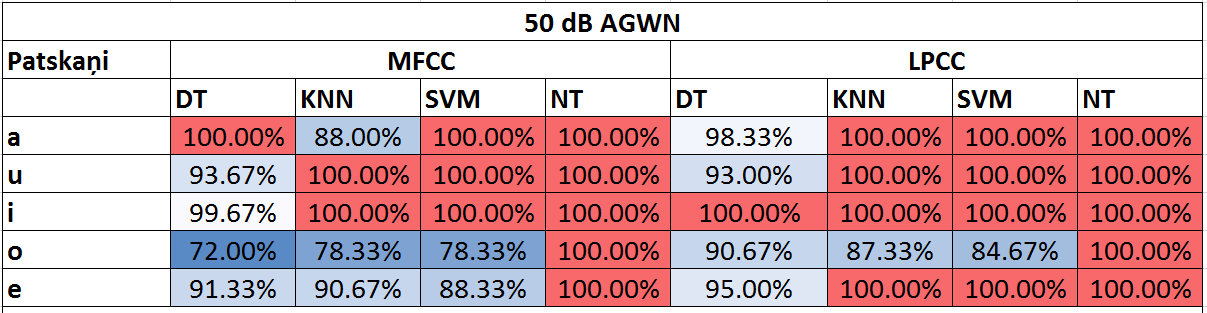
\includegraphics[width=1.00\textwidth, left]{2confussion} 
\label{2confussion} 
\end{table}
 
\begin{table}[H]
\caption{}
\captionsetup{justification=centering}
\caption*{\textbf{Pareizi klasificēto patskaņu rezultātu apkopojums (30 dB)}}
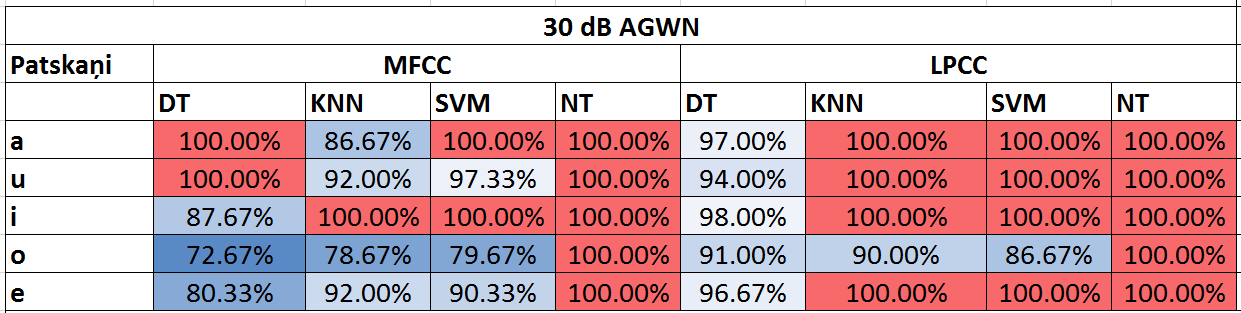
\includegraphics[width=1.00\textwidth, left]{0confussion} 
\label{0confussion} 
\end{table}

\begin{table}[H]
\caption{}
\captionsetup{justification=centering}
\caption*{\textbf{Pareizi klasificēto patskaņu rezultātu apkopojums (20dB)}}
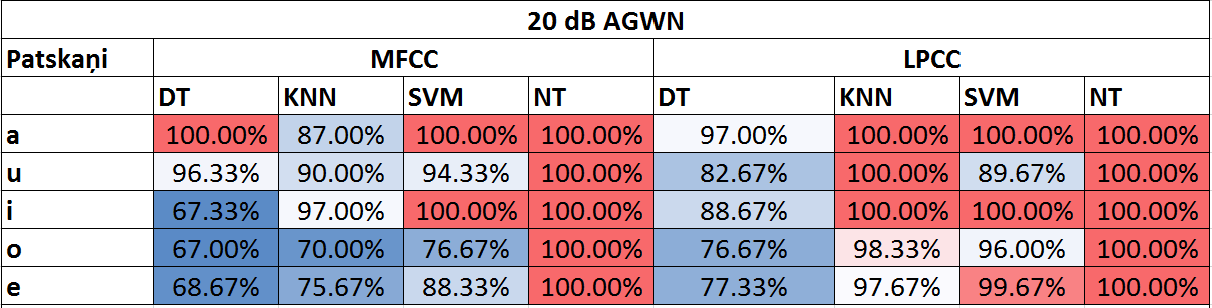
\includegraphics[width=1.00\textwidth, left]{1confussion} 
\label{1confussion} 
\end{table}

\begin{table}[H]
\caption{}
\captionsetup{justification=centering}
\caption*{\textbf{Pareizi klasificēto patskaņu rezultātu apkopojums (10dB)}}
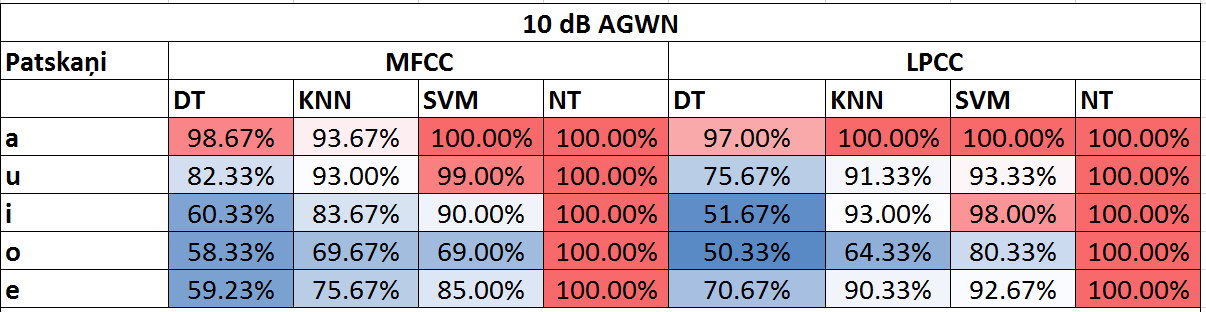
\includegraphics[width=1.00\textwidth, left]{3confussion} 
\label{3confussion} 
\end{table}

No iegūtajiem datiem var novērot to, ka palielinoties 
signāla-trokšņa attiecībai klasifikatoru SVM, KNN, DT 
veiktspēja pieaug izmantojot gan LPCC, gan MFCC.

Pievienojot Gausa balto troksni skaņas signāliem, var secināt 
no tabulas datiem, ka vislabākā veiktspēja ir Neironu tīkliem,
bet sliktākā veiktspēja kopumā ir DT klasifikatoram.
Visos gadījumos Neironu tīkli klasificē pareizi visus testa datus.

Kad tiek izmantoti LPCC, vissliktāko veiktspēju kopumā uzrāda DT klasifikators.
Bet izmantojot LPCC, kad SNR ir 50, 30, 20 dB ortu labāko 
veiktspēju uzrāda KNN klasifikators, bet kad SNR ir 10dB, tad labāks ir SVM. 
Kad tiek izmantoti MFCC, otra labākā veiktspēja ir SVM klasifikatoram.

Kopumā labāko veiktspēju SVM un KNN uzrāda, kad SNR ir 30dB izmantojot LPCC.
DT uzrāda kopumā labāko veiktspēju arī, kad SNR ir 30dB, bet
kad tie izmantoti MFCC, un sliktāko veiktspēju kopumā uzrāda, 
kad SNR ir 10dB un tiek izmantoti LPCC. KNN, SVM sliktāko 
veiktspēju kopumā uzrāda, kad SNR ir 10dB un tiek izmantoti MFCC. 

Visprecīzāk klasifikatori SVM, KNN un Neironu tīkli spēj pareizi klasificēt visus patskaņa 'a' testa datus, kad testēšanai un apmācīšanai izmanto LPCC gan pie 10dB, 20dB, 30dB un 50dB lielas signāla-trokšņa attiecības. Pie 30dB un 50dB SNR var novērot to, ka kopumā ļoti labi klasifikatori spēj pareizi klasificēt arī patskaņa 'i' testa datus.
Izmantojot MFCC, gan pie 10dB, 20dB, 30dB un 50dB lielas signāla-trokšņa attiecības klasifikatori SVM, DT un Neironu tīkli spēj pareizi klasificēt visus patskaņa 'a' testa datus, bet klasifikators KNN, pieaugot signāla-trokšņa attiecībai,
spēj visprecīzāk klasificēt visus patskaņa 'i' testa datus. 
Kopumā klasifikatori KNN, SVM, DT izmantojot gan LPCC, gan MFCC, vissliktāk spēja pareizi klasificēt patskaņa 'o' testa datus. 

%\input{secinajumi-un-priesklikumi} %% Ērtāk visu failā secinajumi-un-priesklikumi.tex
%% Nenumurēta nodaļa, kas uzrādās satura rādītājā
\chapter*{Secinājumi un priekšlikumi}
\addcontentsline{toc}{chapter}{Secinājumi un priekšlikumi}
\begin{enumerate}
\item MATLAB vide ir viegli izmantojama, ar labu dokumentāciju un piemērota, lai varētu veikt skaņas signālu apstrādi, analīzi, kā arī īpašību izgūšanu un klasifikatoru veiktspējas testēšanu. 
\item Jo lielāka signāla-trokšņa attiecība, jo labāka ir klasifikatoru SVM, DT, KNN veiktspēja.
\item Neironu tīkli klasificē pareizi visus testa datus pie 10, 20, 30, 50dB Gausa baltā trokšņa signāla-trokšņa attiecības, kad testēšanai un apmācīšanai izmanto MFCC vai LPCC. 
\item Izmantojot apmācīšanai un klasifikācijai LPCC pie dažādiem trokšņu līmeņiem, klasifikatoriem kopumā ir labāka veiktspēja, nekā izmantojot MFCC pie dažādiem trokšņu līmeņiem. 
\item Klasifikatori SVM, KNN, DT slikti spēj pareizi klasificēt tādus patskaņus kā 'o', bet labi spēj pareizi klasificēt tādus patskaņus kā 'a','i'.
\item Ar ierunātajiem skaņas signāliem ir par maz, lai varētu veikt klasifikāciju. Ir nepieciešams izveidot daudz vairāk realistiskus testa datus latviešu valodā.
\item Izveidot sintētisku skaņas signālu ir viegli, pietiek tikai zināt patskaņa F1, F2. 
\item Tālākajos pētijumos var izmantot TensorFlow un programmēšanas valodu Python, lai ar Neironu tīklu palīdzību veiktu patskaņu atpazīšanu izrunātajos vārdos vai teikumos. 
\item Tika apskatīts, kā veidojas angļu valodas patskaņi. Noderīgi būtu veikt izpēti par
latviešu valodas patskaņiem. Gan par anatomiskajām īpatnībām izrunājot patskaņus, gan 
par formantām, kas veido katru izrunāto patskani.
\item Balstoties uz rezultātiem, kas iegūti ģenerējot sintētiskus datus, var spriest par optimālu algoritmu izvēli, ko pielietot reāliem datiem.
\end{enumerate}


\chapter*{Izmantotās literatūras un avotu saraksts}

\title{References}
\begingroup
   \def\chapter*#1{}
   \addcontentsline{toc}{chapter}{Izmantotās literatūras un avotu saraksts}
\bibliography{bib/library}
\bibliographystyle{IEEEtran}
\endgroup

% \printbibliography[title={Reference}]
%\printbibliography
\appendix
\chapter*{Pielikumi}
\addcontentsline{toc}{chapter}{Pielikumi}

\section{Metode divu signālu salīdzināšana (MATLAB)}
\label{appendix:piel1}
\begin{lstlisting}
function [dist,nor] = soundCompare(sample1, sample2)
%Ielasa audio signalu
[signal_1, fs_1] = audioread(char(sample1));
[signal_2, fs_1] = audioread(char(sample2));
%Veic troksnu  filtraciju
s1_f = WienerScalart96(signal_1,fs_1);
s2_f = WienerScalart96(signal_2,fs_1);
%Tiek veikta fona troksnu un klusumu iznemsana
[segments1, fs] = detectVoiced(s1_f, fs_1);
[segments2, fs] = detectVoiced(s2_f, fs_1);

s1_fd = segments1{:};
s2_fd = segments2{:};

%Tiek vekta digitala laika deformacija
d2x = dtw(s1_fd,s2_fd, fs_1);
%mfcc metodi izmanto no Audiotoolbox
[ceps1,freqresp1,fb1,fbrecon1,freqrecon1]=mfcc(s1_fd,fs_1);
[ceps2,freqresp2,fb2,fbrecon2,freqrecon2]=mfcc(d2x,fs_1);

features1 = ceps1(2:end,:);
features2 = ceps2(2:end,:);
%Veic distancu aprekinasanu izmantojot Eiklida un Bhattacharyya distanci
dist = bhattacharyya(features1(:),features2(:));
nor = norm(features1-features2);
end
\end{lstlisting}
\section{Skripts skaņas signāla ierakstīšanai (MATLAB)}
\label{appendix:piel2}
\begin{lstlisting}
fs = 16000; %izgusanas frekvence
nBits = 24;
nChannels = 1;

recorder = audiorecorder(fs, nBits, nChannels); %uzstada audio ierakstitajam parametrus

T =2; %Laiks sekundes
recordblocking(recorder,T); %uzstada ierakstisanas ilgumu 
y = getaudiodata(recorder); %izveido audio ierakstitaju

filename = 'file_name.wav';

audiowrite(filename,y,fs) %ieraksta audio failu

play(recorder) %atskano audio failu 

t = 1/fs:1/fs:T; %laika intervails
plot(t,y); %Izveido ieguta skanas signala grafiku
 \end{lstlisting}
 
 
 
  \section{Skaņas signāla īpašību izgūšana izmantojot dažādus koeficientus (MATLAB)}
\label{appendix:piel3}
\begin{lstlisting}
 function XDATA= cepstral(dire, cepstralCoefficients)
%*********************************************************************%
%Ievade:
%dire - skanas signalu direktorija 
%cepstralCoefficients - mainigais nosaka, kuru metodi izmantot
%Cepstralo koeficientu iegusanai:
%           1 - LPCC
%           2 - Rasta-PLP
%           3 - MFCC
%Izvade:
%XDATA - cepstralo koeficentu matrica katram skanas signalam
%*********************************************************************%
    wav_folder = {dire};
    %Atrod visus wav failus attiecigaja direktorija
    for i = 1:length(wav_folder)
        aa = dir(fullfile(wav_folder{i}, '*.wav'));
    end
    
    for kk = 1:length(aa)
        %atrod audio faila nosaukumu
        acq_fn_1 = fullfile(wav_folder{i}, aa(kk).name);
        %Ielasa audio failu 
        [Samples, fs] = audioread(acq_fn_1);
        %Pielieto troksnu filtresanu 
        s1_f = WienerScalart96(Samples,fs);
        
        %Iegust signala ipasibu koeficientus izmantojot attiecigo metodi
        if cepstralCoefficients ==1
            ceps1=msf_lpcc(s1_f, fs,'order',10);
        elseif cepstralCoefficients ==2
            ceps1=rastaplp(s1_f, fs, 1, 12);
        elseif cepstralCoefficients == 3
            ceps1=msf_mfcc(s1_f,fs);
        end
        %Izveido matricu, kuru aizpilda ar nullem
        if kk ==1
            [x,y]=size(ceps1);
            x=x-1;
            XDATA = zeros(x*y,length(aa));
        end
        %atmet pirmo rindu
        cepsc = ceps1(2:end,:);
        %Ievieto signala ipasibu koeficientus matrica
        XDATA(:,kk) = cepsc(:);
    end    
end
\end{lstlisting}
 
\section{KNN Klasifikatora apmācība (MATLAB)}
\label{appendix:piel4}
\begin{lstlisting}
 function KNNstruct = trainClasificator(trainingSamples,cepstrum)
%*********************************************************************
%INPUT:
%trainingSamples - katras klases apmacibai izmantoto skanas signalu skaits
%cepstrum - mainigais nosaka, kuru metodi izmantot cepstralo koeficientu iegusanai:
%           1 - LPCC
%           2 - Rasta-PLP
%           3 - MFCC
%OUTPUT
%KNNstruct - satur informaciju  par apmacito klasifikatoru 
%*********************************************************************
%Tiek vekta skanas signalu ipasibu koeficientu izgusana
%Tiek noradita direktorija no kuras nem attiecigos skanas signalus
XDATAC = cepstral('C:\Users\user\Documents\sound files\C',cepstrum);
XDATAFive =cepstral('C:\Users\user\Documents\sound files\Five',cepstrum);
XDATAPoint = cepstral('C:\Users\user\Documents\sound files\Point',cepstrum);
XDATAV = cepstral('C:\Users\user\Documents\sound files\V',cepstrum);
XDATAA= cepstral('C:\Users\user\Documents\sound files\A',cepstrum);
XDATAB= cepstral('C:\Users\user\Documents\sound files\B',cepstrum);
%Izveido matricas, kas satur katras klases ipasibu koeficientus
At = XDATAA(:,1:trainingSamples);
Bt = XDATAB(:,1:trainingSamples);
Ct = XDATAC(:,1:trainingSamples);
Fivet = XDATAFive(:,1:trainingSamples);
Pointt = XDATAPoint(:,1:trainingSamples);
Vt = XDATAV(:,1:trainingSamples);
%Visus datus saliek viena mainigaja
X_train = [At, Bt, Ct, Fivet, Pointt, Vt]';
%nodefine piecas klases
twos(1,1:trainingSamples) = 2;
threes(1,1:trainingSamples) = 3;
fours(1,1:trainingSamples) = 4;
fives(1,1:trainingSamples) = 5;
zeros(1,1:trainingSamples) =0;
ones(1,1:trainingSamples) =1;
%Izveido vektoru, kas satures klasu nosaukumus 
labels_t = [zeros, ones, twos, threes,fours, fives];
%Veic apmacibu izmantojot KNN klasifikatoru
KNNstruct = fitcknn(X_train,labels_t);
end
\end{lstlisting}

\section{KNN Klasifikatora testēšanas metode (MATLAB)}
\label{appendix:piel5}
\begin{lstlisting}
function [labels_s, groupIDs,confusionMat] = testClasificator(testSamples, traingingSamples,cepstrum,sampledir1,sampledir2,sampledir3, sampledir4, sampledir5, sampledir6)
%*********************************************************************
%INPUT:
%testSamples -  katras klases testesanai izmantoto skanas signalu skaits
%trainingSamples -  katras klases apmacibai izmantoto skanas signalu skaits
%cepstrum - mainigais nosaka, kuru metodi izmantot cepstralo koeficientu iegusanai
%           1 - LPCC
%           2 - Rasta-PLP
%           3 - MFCC
%sampledir1, sampledir2, sampledir3, sampledir4, sampledir5, sampledir6
% - direktorijas, kas norada no kurienes tiek nemti skanas signali
% testesanai
%OUTPUT
%labels_s - matrica, kas norada pie kuras klases patiesi pieder skanas
%signals
%groupIDs - matrica, kas parada klasifikatora veikto skanas signalu
%klasifikaciju
%confusionMat - kludas matrica
%*********************************************************************
%Tiek vekta skanas signalu ipasibu koeficientu izgusana
%Tiek noradita direktorija no kuras nem attiecigos skanas signalus
XDATA= cepstral(sampledir1,cepstrum);
XDATB= cepstral(sampledir2,cepstrum);
XDATAC = cepstral(sampledir3,cepstrum);
XDATAFive =cepstral(sampledir4,cepstrum);
XDATAPoint = cepstral(sampledir5,cepstrum);
XDATAV = cepstral(sampledir6,cepstrum);

%Izveido matricas, kas satur katras klases ipasibu koeficientus
As = XDATA(:,1:testSamples);
Bs = XDATB(:,1:testSamples);
Cs = XDATAC(:,1:testSamples);
Fives = XDATAFive(:,1:testSamples);
Points = XDATAPoint(:,1:testSamples);
Vs = XDATAV(:,1:testSamples);
%Iegust apmacitu klasifikatoru 
KNNstruct= trainClasificator(traingingSamples,cepstrum);
%Visus mstricu datus saliek viena mainigaja
X_sample = [As, Bs, Cs, Fives, Points, Vs]';
%nodefine piecas klases
twos(1,1:testSamples) = 2;
threes(1,1:testSamples) = 3;
fours(1,1:testSamples) = 4;
fives(1,1:testSamples) = 5;
zeros(1,1:testSamples) =0;
ones(1,1:testSamples) =1;
%Izveido vektoru, kas satures klasu nosaukumus 
labels_s = [zeros, ones, twos, threes,fours, fives];
%Veic testesanu izmantojot testa skanas signalu ipasibas un apmacito
%klasifikatoru, iegustot minejumu matricu 
groupIDs = predict(KNNstruct, X_sample);

labels_s = labels_s';
%Iegust kludas matricu 
confusionMat = confusionmat(groupIDs,labels_s);
end
\end{lstlisting}


\chapter*{Galvojums}
\sloppy
\addcontentsline{toc}{chapter}{Galvojums}
 
 Ar šo es, \defAutors, galvoju, ka bakalaura darbs ir izpildīts patstāvīgi, konsultējoties ar darba vadītāju. No svešiem pirmavotiem ņemtā informācija ir norādīta ar atsaucēm, dati un definējumi ir uzrādīti darbā. Šis darbs tādā vai citādā veidā nav nekad iesniegts nevienai citai pārbaudījumu komisijai. 
 
Esmu informēta, ka mans bakalaura darbs tiks ievietots un apstrādāts Vienotajā datorizētajā plaģiāta kontroles sistēmā plāģiāta kontroles nolūkos.
 
\vspace{1in}
2017.gada \rule{1cm}{0.2pt} \hspace{0.4cm}\rule{3cm}{0.2pt} \hspace{3.6cm}\rule{5cm}{0.2pt} \hspace*{12.5cm}\textit{\raisebox{1em}{(paraksts)}}

\label{LastPage}

\end{document}




